\documentclass[11pt,letterpaper]{article}
\usepackage{lmodern}
\usepackage{authblk}
\usepackage{tabularx,booktabs}
\usepackage{graphicx}
\usepackage[utf8]{inputenc}
\usepackage[margin=1.0in]{geometry}
\usepackage[hidelinks]{hyperref}
\usepackage[T1]{fontenc}
\usepackage[utf8]{inputenc}
\usepackage{amsmath,amssymb}
\usepackage{placeins}
\usepackage{url}
\setlength{\marginparwidth}{2cm}
\usepackage[labelfont=bf]{caption}



\usepackage{amsmath,amssymb}

\newcommand{\junk}[1]{}
\usepackage{float}
\let\footnotesize\small
\setlength{\textfloatsep}{10pt plus 2pt minus 2pt}
\setlength{\floatsep}{8pt plus 2pt minus 2pt}
\setlength{\intextsep}{8pt plus 2pt minus 2pt}
\setlength{\emergencystretch}{2em}
\renewcommand{\topfraction}{0.9}
\renewcommand{\bottomfraction}{0.8}
\renewcommand{\textfraction}{0.08}
\begin{document}
\thispagestyle{empty}

%\title{RECOMB paper template}
\title{MeBench: Benchmarking Biological Mechanism Reasoning in Language Models through TF-to-Gene Regulation}
\setcounter{Maxaffil}{2}
\author[1]{Haochuan Wang\thanks{%
These authors contributed equally to this work. Emails:
Haochuan Wang (\href{mailto:hw106@illinois.edu}{hw106@illinois.edu});
Tianzuo Yuan (\href{mailto:uc31642@um.edu.mo}{uc31642@um.edu.mo});
Yurui Li (\href{mailto:yuruil2@illinois.edu}{yuruil2@illinois.edu}).
}}

\author[2]{Tianzuo Yuan\protect\footnotemark[1]}
\author[1]{Yurui Li\protect\footnotemark[1]}
\author[1]{Dehao Wu}

\author[1]{Xiaopeng Yuan}
\author[1]{Peng Kuang}
\author[4]{Jingxuan Bao}
\author[5]{Shizhuo Mu}
\author[3]{Yang Li}
\author[1]{Haohan Wang\thanks{Corresponding author. Email: \href{mailto:haohanw@illinois.edu}{haohanw@illinois.edu}.}}
%\author[1,2,\thanks{Corresponding author. Email: \href{thirteenth@doctorwho.com}{thirteenth@doctorwho.com}}]{}
\affil[1]{\small School of Information Science, University of Illinois at Urbana-Champaign}
\affil[2]{\small Faculty of Science, University of Macau}
\affil[3]{\small Department of Ecology and Evolutionary Biology, University of Michigan, Ann Arbor}
\affil[4]{\small Brown University}
\affil[5]{\small Department of Bioengineering, University of Pennsylvania}
\date{}

\maketitle

\begin{abstract}
  Predicting the direction of a target gene after perturbation does not establish that a model can identify the underlying regulatory mechanism. We introduce a benchmark for transcription factor (TF)-to-gene regulation that integrates mechanism-specific experimental evidence. We evaluate whether models make accurate predictions and provide concise mechanistic explanations. We developed a benchmark comprising three tasks. Task 1 assesses mechanism classification using 171 TF-to-gene pairs assigned to four regulatory categories: direct cis-regulatory DNA, chromatin-mediated regulation, combinatorial TF regulation and regulatory RNA-mediated regulation. We curated regulatory mechanisms and then matched perturbations for task 2, yielding 193 forward-reasoning units, and constructed task 3 that includes inverse-intervention units from different perturbation types for the same TF-to-gene pairs. Tasks 2 and 3 also evaluate the mechanistic explanations supporting model predictions. Explanations are assessed for mechanism, mediator, causal role and order, intervention-to-outcome logic, and consistency with curated evidence. Across six evaluated systems, Task 1 macro-F1 and Task 2/3 joint F1 scores range from 22.7\% to 34.5\% for Task 1, 57.5\% to 78.4\% for Task 2, and 25.6\% to 35.7\% for Task 3. Full-chain reasoning pass rates range from 62.0\% to 84.7\% in forward reasoning of Task 2 and 43.8\% to 72.5\% in inverse reasoning of Task 3. The evaluated systems show recurring difficulties in recovering required regulatory dependencies and their context-specific causal roles. These results identify specific weaknesses in evidence-aligned mechanistic explanations under the benchmark conditions. 
%Our benchmark provides a focused behavioral assessment of biological mechanism understanding.

\par\medskip
\noindent\textbf{Keywords:} TF-to-gene regulation; perturbation responses; LLMs' mechanistic reasoning

\end{abstract}

\clearpage
\section{Introduction}
  
Interpreting biological mechanisms requires identifying the functional roles of molecular components and explaining how their interactions produce a response. A transcription factor (TF) may regulate its target genes by acting at cis-regulatory elements, relying on chromatin regulators, cooperating with other TFs or regulating RNA intermediates~\cite{dong2025znf143,gallant2012deltanp63alpha,biddie2011transcription,yoshioka2012micromanaging}. Evaluating a model's ability to identify TF-to-gene regulatory mechanisms is therefore essential when assessing its suitability for interpreting perturbation experiments. Different regulatory mechanisms can produce the same direction of expression change. Consequently, correctly predicting whether a target gene is upregulated or downregulated does not establish that a model has identified the mechanism responsible for that response.

Existing works evaluated related aspects of biological prediction. BEELINE evaluates gene regulatory network reconstruction~\cite{pratapa2020benchmarking}, GEARS predicts transcriptional responses to multi-gene perturbations~\cite{roohani2024predicting}, PerturbQA asks questions about perturbation experiments~\cite{wu2025contextualizing}.  These tasks assess regulatory relationships or perturbation outcomes, but their prediction targets do not require identifying the specific molecular mechanism underlying an individual TF–gene relationship. PertReason directly evaluates cell-state-conditioned mechanistic explanations using perturbation data and knowledge-graph paths~\cite{kim2026pertreason}. CellChain tests how predictions depend on controlled changes in cross-scale evidence~\cite{xia2026cellchain}. These approaches provide valuable assessments of pathway reconstruction and evidence use. MeBench complements these evaluations by distinguishing experimentally supported modes of TF--gene regulation and testing the required components and their causal roles in both forward and inverse intervention reasoning. 

%Addressing this question requires reference annotations that explicitly connect each regulatory category to the experimental evidence supporting its mediator and causal dependencies. For each regulatory pair in our benchmark, explicit experimental evidence requirements define the reference category, mediator and causal dependencies. Complementary intervention tasks then assess the models’ understanding of these mechanisms.

We assess models’ mechanistic understanding through the content of their answers. Each model must identify the experimentally supported regulatory mechanism, explain the role of the required mediator and the relevant causal relationships, and use these relationships to explain the response to a perturbation. An answer that names the correct molecules but reverses their roles does not meet these criteria. Neither does a correct prediction of response direction without the required mechanistic explanation. We collected evidence from published studies to support this assessment. TF occupancy suggests a potential regulatory interaction, but binding alone does not demonstrate an effect on gene expression~\cite{cusanovich2014functional}. Targeted enhancer perturbations can establish functional links between regulatory elements and their target genes~\cite{fulco2019activity}, while genome-scale Perturb-seq measures expression responses to genetic perturbations~\cite{replogle2022mapping}. Identifying the mechanism behind a response requires further evidence showing how the relevant molecular components contribute to that response and which factors or interactions are necessary~\cite{gallant2012deltanp63alpha}. These distinctions form the basis of the evidence requirements for each regulatory mechanism in our benchmark.

The MeBench evaluates models’ ability to reason about regulatory mechanisms through three tasks. Task 1 asks models to identify how the TF regulates its target gene. Task 2 requires them to apply that mechanism to predict and explain the target gene’s response to a given perturbation. Task 3 requires inverse reasoning: inferring the perturbation type from the response direction and the perturbed entity. A shared five-criterion rubric evaluates the mechanistic reasoning in Tasks 2 and 3. Joint correctness requires both a correct task-specific answer and an explanation that satisfies all five criteria; a correct prediction alone is therefore insufficient for full credit. We evaluated six models using 171 curated TF–to-gene pairs. We assessed their mechanistic understanding from their responses to the given inputs, focusing on their ability to apply biological knowledge to identify regulatory mechanisms and explain perturbation responses. Evaluation results revealed that current LLMs have limitations in identifying regulatory mechanisms of molecular components. In the forward and inverse reasoning tasks, models sometimes identified the relevant molecules but incorrectly characterized functions. Under the benchmark conditions, the evaluated systems do not consistently recover the evidence-supported dependencies connecting regulatory components to target responses.









   
\section{Methods}
  \subsection{Design and construction of Mebench}
Evaluating models’ ability to identify and reason about regulatory mechanisms requires reference annotations that specify how a TF regulates its target gene and document the supporting experimental evidence. We therefore curated TF–gene relationships from published experimental studies. Each entry describes the TF–gene pair, its regulatory mechanism, and the evidence supporting that mechanism. The record includes validated contexts, references and source locations, the key feature required for the assigned mechanism category, mediator information and checks against all four candidate mechanisms (Figure~\ref{fig:benchmark_overview}).

The direct cis-regulatory DNA category requires TF occupancy at a promoter, enhancer or other cis-regulatory element linked to the target gene, together with functional evidence of TF-dependent target regulation. Functional evidence may come from perturbing either the TF or the regulatory element; the element itself need not be perturbed in every case. Occupancy, motif presence or an expression association alone is insufficient. Pairs are excluded if experimentally demonstrated dependencies meet the criteria for one of the other three categories. Chromatin-mediated regulation requires a specified chromatin state, modification, nucleosome process, or regulator whose necessity for TF occupancy, TF-dependent cis-regulatory activity, or the TF-dependent target response is demonstrated by perturbation, rescue, or an equivalent dependency test. Correlated accessibility or histone-mark changes do not alone establish this label. Combinatorial TF regulation requires a specified partner TF whose cooperation, competition, or antagonism is necessary for the target response, supported by individual or joint perturbation, interaction disruption, rescue, or an equivalent functional test. Regulatory RNA-mediated regulation requires a TF-to-RNA-to-target relay involving a named miRNA or lncRNA. The specified admission criteria require support for both links and the intermediate’s necessity through perturbation, rescue, or an equivalent dependency test. This regulation can affect RNA stability or translation. We therefore assign response labels according to the target-expression readout measured in the source study. After confirming the regulatory mechanism for each pair, we matched perturbation experiments conducted in compatible experimental contexts, with clearly defined perturbation–control comparisons and unambiguous measured responses of the target gene. The direction of change in target gene expression was defined relative to the corresponding control. The released source table contains the perturbation records. We also recorded the experimental methods, control conditions, doses, time points, assays and source locations. 
\begin{figure}[!t]
  \centering
  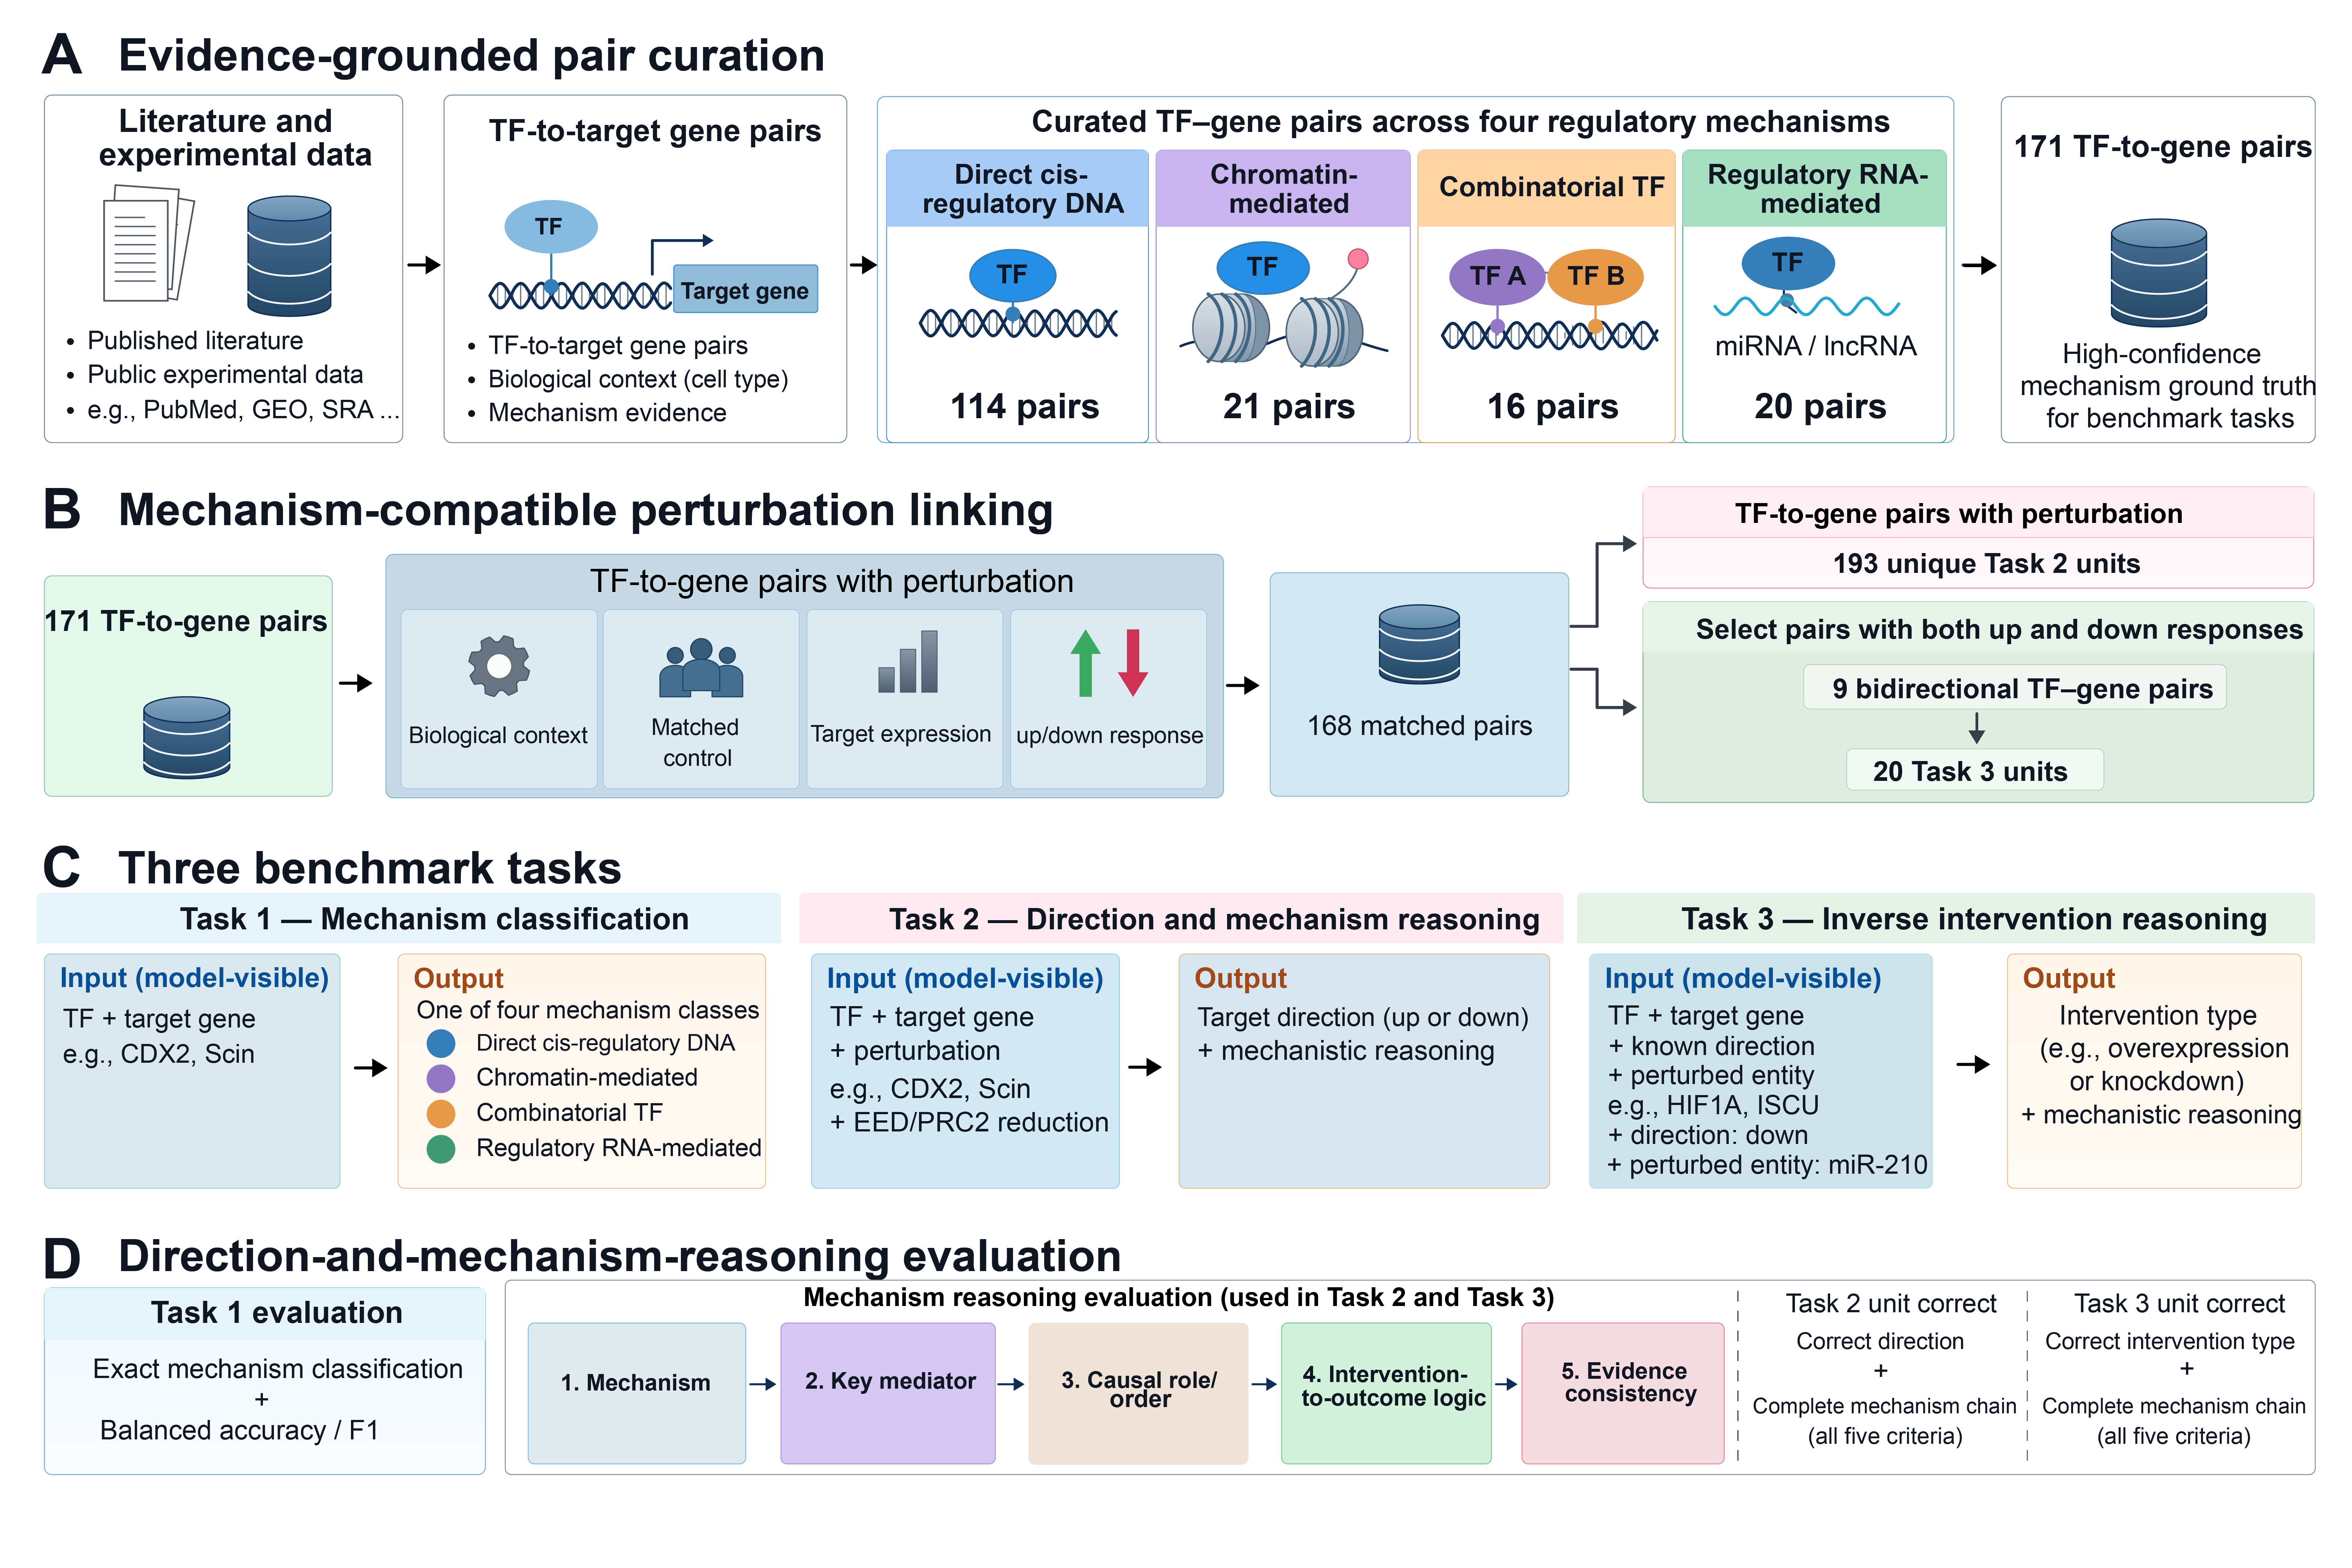
\includegraphics[width=0.85\linewidth]{figs/Fig_1-01.png}
  \captionsetup{skip=2pt}
  \caption{Construction and evaluation of MeBench.
  The benchmark contains 171 accepted TF-to-gene pairs, 193 evaluation units in Task 2, and 20 Task 3 units based on different perturbation types for the same TF-to-gene pairs. The three tasks assess mechanism identification, forward mechanistic reasoning and inverse mechanistic reasoning.}
  \label{fig:benchmark_overview}
\end{figure}



Task 1 includes 171 TF-to-gene pairs: 114 assigned to direct cis-regulatory DNA, 21 to chromatin-mediated regulation, 16 to combinatorial TF regulation and 20 to regulatory RNA-mediated regulation. Task 2 comprises 193 evaluation units covering 168 TF-to-gene pairs, including 112 direct cis-regulatory DNA, 20 chromatin-mediated, 35 combinatorial TF and 26 regulatory RNA-mediated units. Of these, 167 are labelled down and 26 up. Task 3 contains 20 evaluation units across nine TF-to-gene pairs, with 10 units each for combinatorial TF and regulatory RNA-mediated regulation (Figure~\ref{fig:unit_number}).

\begin{figure}[!htbp]
  \centering
  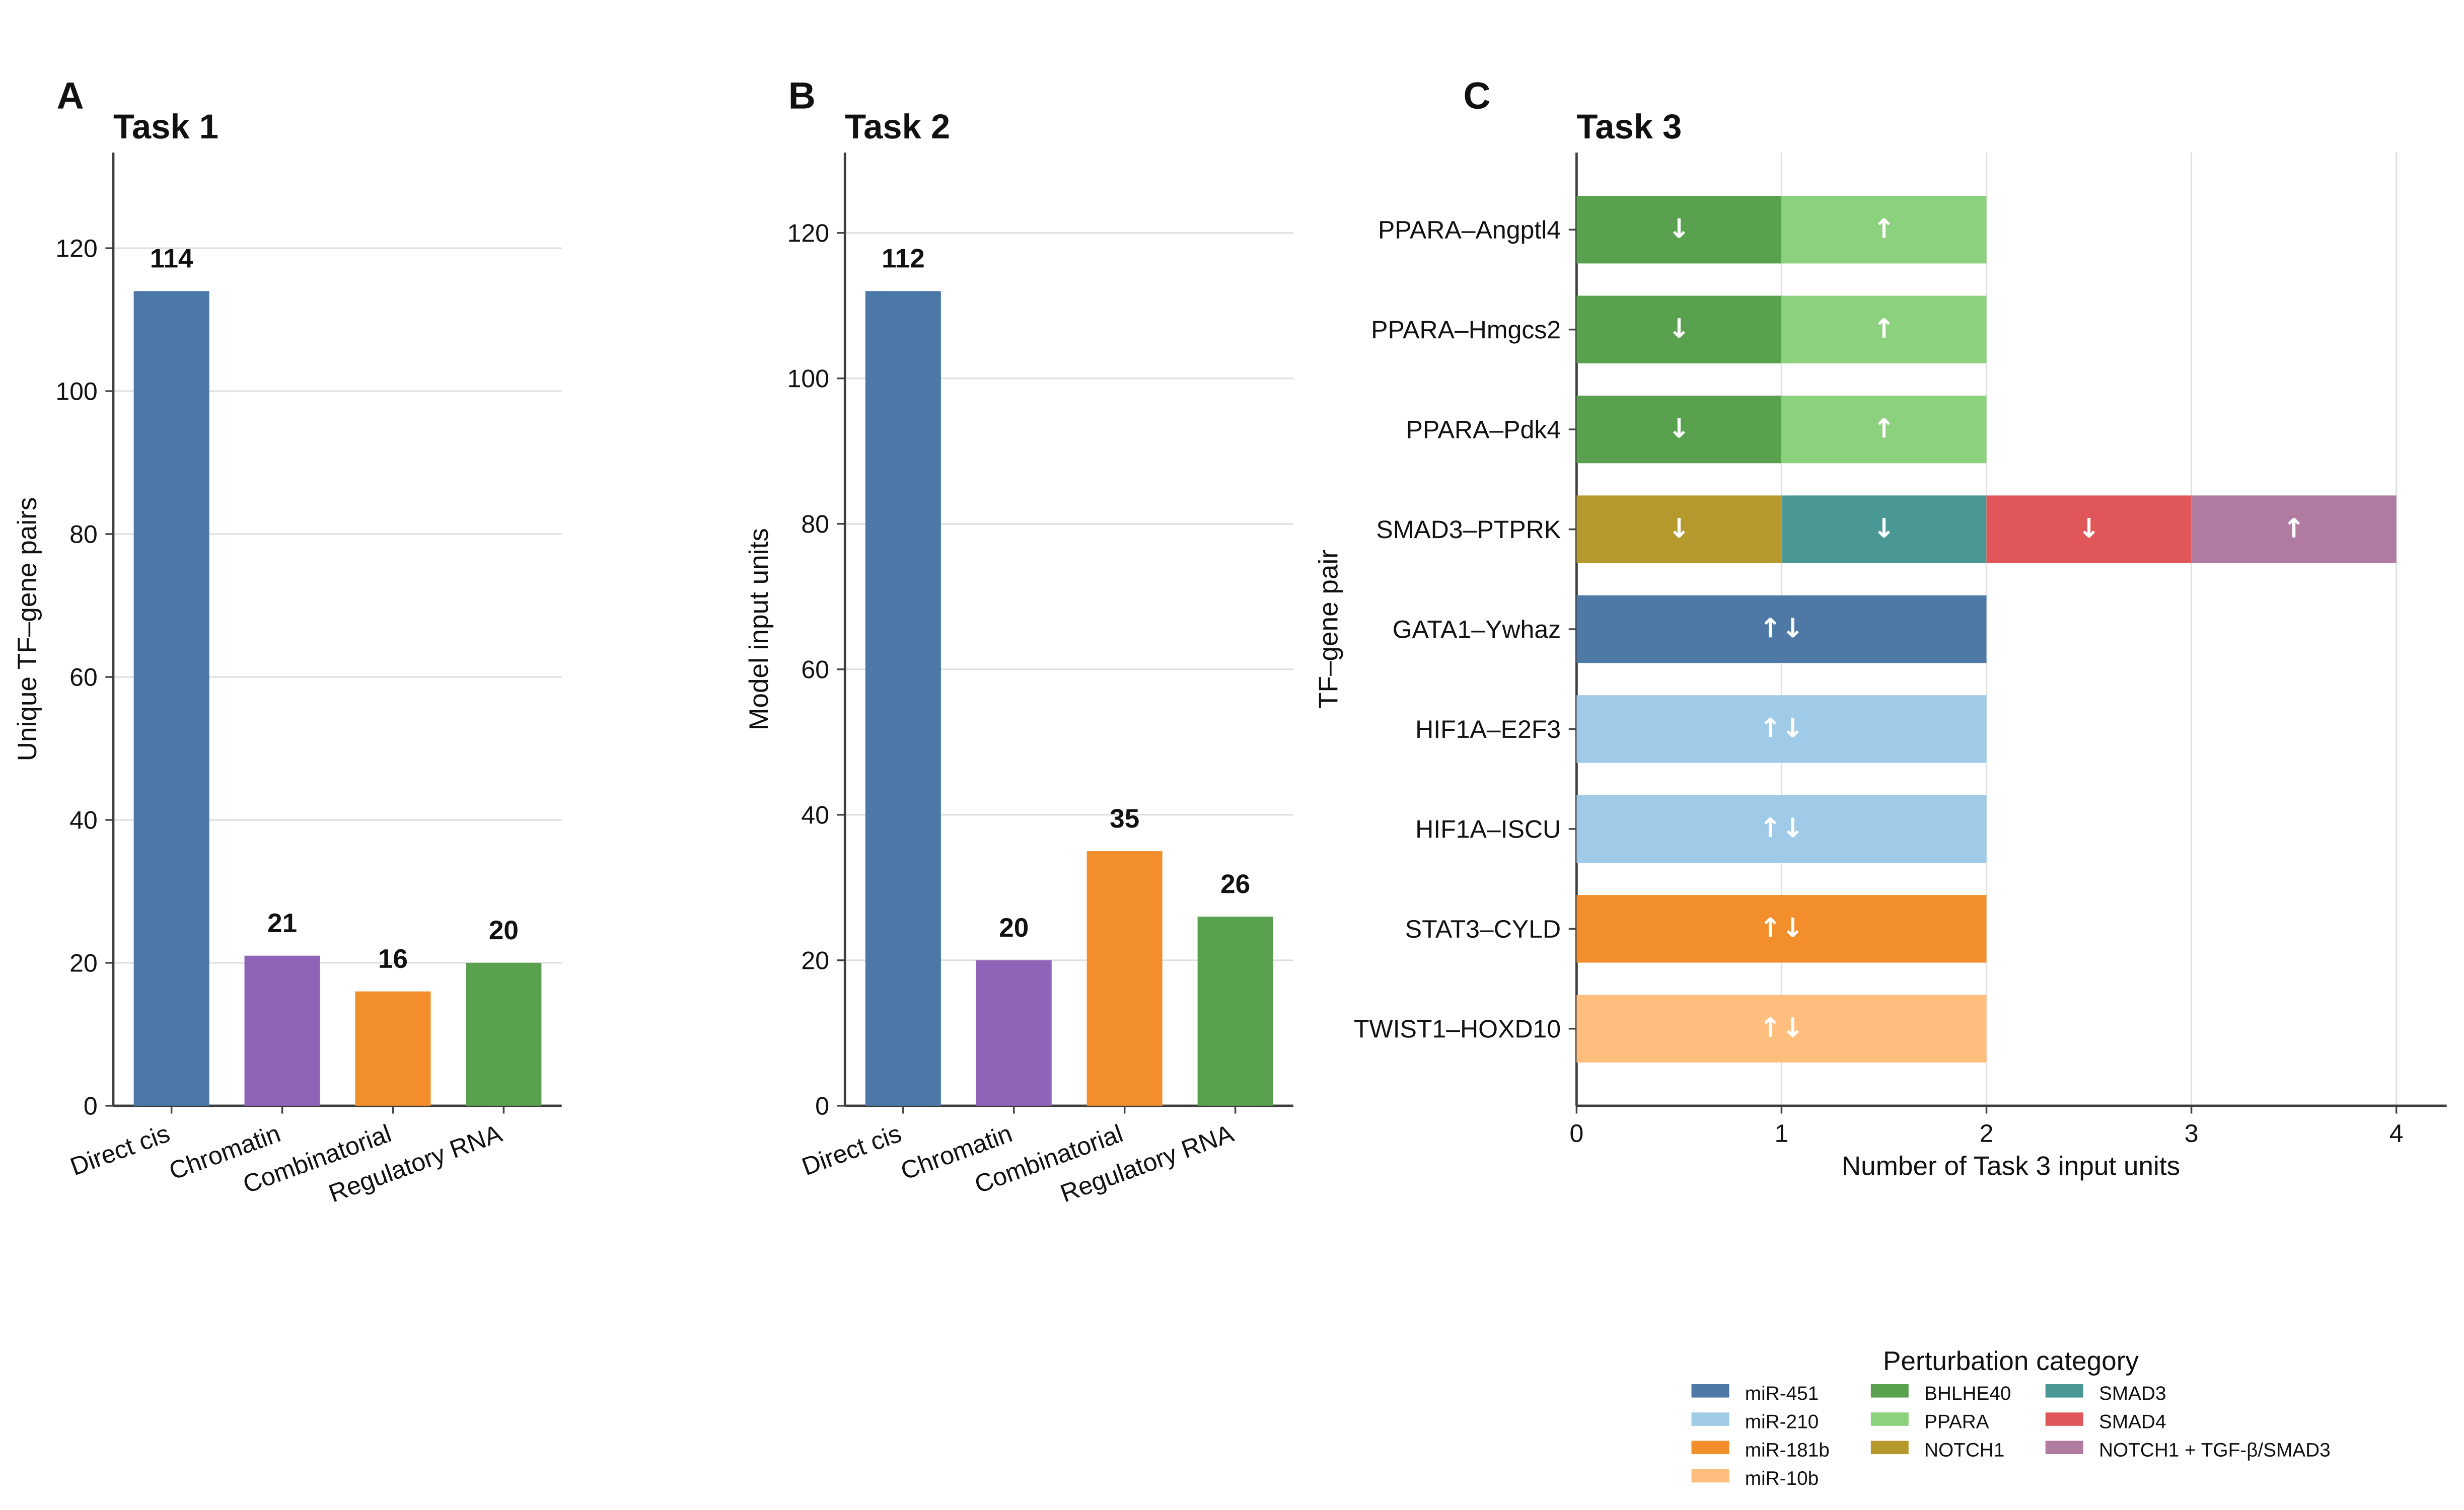
\includegraphics[width=0.82\linewidth]{figs/Fig_2.png}
  \captionsetup{skip=2pt}
  \caption{Number of the evaluation units in each task.
  (A) Distribution of 171 unique TF--gene pairs across four regulatory mechanisms in Task 1.
  (B) Distribution of 193 input units across four regulatory mechanism categories in Task 2.
  (C) Composition of 20 input units spanning nine TF--gene pairs in Task 3.}
  \label{fig:unit_number}
\end{figure}



\subsection{Benchmarking methods}

Task 1 provides only the TF and target gene and asks models to select one of the four mechanism labels. Biological context, perturbations, expression measurements, source information and curator notes are withheld. Task 2 provides TF, target gene, and the perturbation and asks for an up/down prediction and one concise mechanistic reasoning in natural language. Task 3 supplies the TF, target, response direction, and perturbed entity, and requests an intervention type and reasoning. The nine pairs have documented responses in both directions under different perturbations (Figure~\ref{fig:task_input}).

\begin{figure}[!htbp]
  \centering
  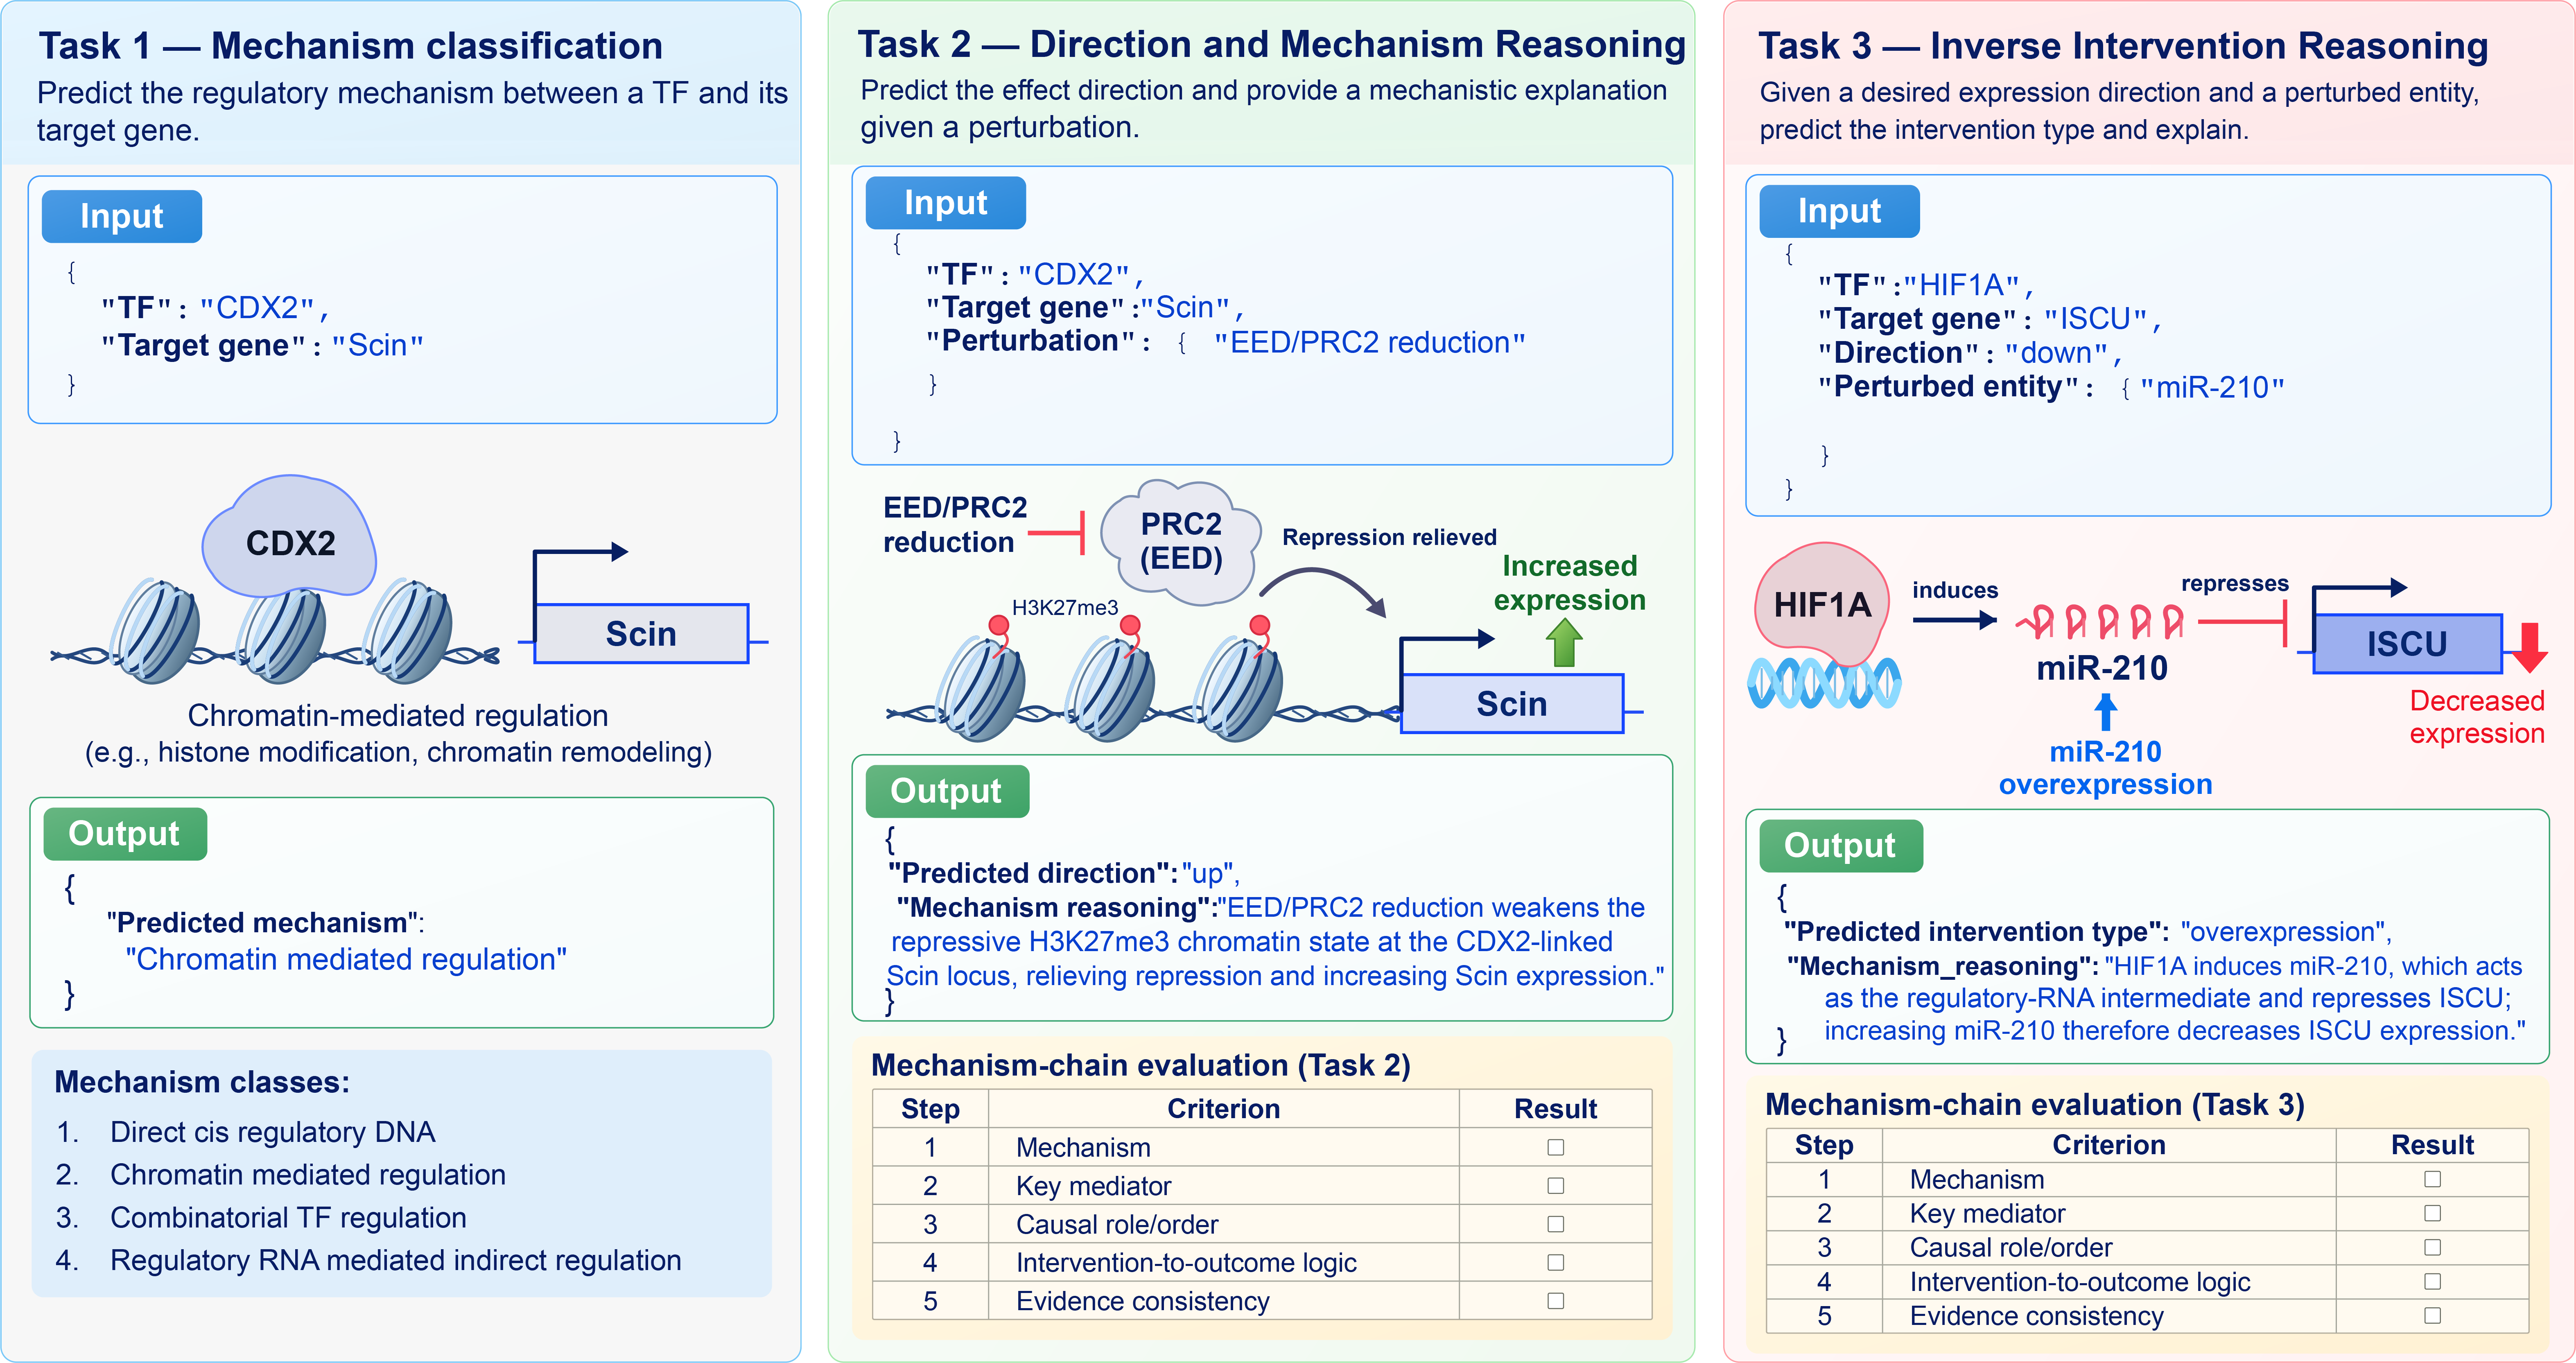
\includegraphics[width=0.85\linewidth]{figs/Fig_3.png}
  \captionsetup{skip=2pt}
  \caption{Examples of tasks' inputs and outputs.}
  \label{fig:task_input}
\end{figure}






We assessed models’ mechanistic reasoning using five criteria: mechanism correctness, mediator correctness, causal role and order, intervention-to-outcome logic, and evidence consistency. Mechanism correctness assesses whether the reasoning identifies the experimentally supported regulatory category for the TF–gene relationship. Mediator correctness evaluates whether it identifies the key component required for that mechanism, such as a chromatin regulator, partner TF, or regulatory RNA. Causal role and order assesses whether the reasoning correctly assigns activating or repressive functions to the relevant components and places them in the appropriate causal sequence. Intervention-to-outcome logic evaluates whether the explanation correctly connects the supplied perturbation in Task 2, or the inferred intervention in Task 3, to the target gene’s response direction. Finally, evidence consistency checks whether the reasoning makes claims that conflict with the curated experimental evidence, including incorrect molecular interactions, functional roles, or regulatory effects. The mechanistic reasoning passes the full-chain evaluation only when all five criteria are satisfied ~\eqref{eq:mechanism_scoring}. 

\begin{equation}
\label{eq:mechanism_scoring}
C_i = \prod_{k=1}^{5} r_{ik},
\qquad
J_i^{(2)} = \mathbb{1}\!\left[\hat{y}_i = y_i\right] C_i,
\qquad
J_i^{(3)} = \mathbb{1}\!\left[v(\hat{a}_i) \in A_i\right] C_i.
\end{equation}

Here, \(i\) indexes evaluation units and \(k\) indexes the five explanation criteria. The binary judgment \(r_{ik}\) indicates whether unit \(i\) satisfies criterion \(k\), and \(C_i=1\) only when all five criteria are met. For Task 2, \(y_i\) and \(\hat{y}_i\) denote the reference and predicted target-gene response directions, respectively. For Task 3, \(\hat{a}_i\) denotes the predicted intervention type, \(v\) is the string-normalization function used by the scorer, and \(A_i\) contains the accepted intervention types for the supplied entity and response direction, with each reference type normalized using \(v\). The indicator function \(\mathbb{1}[\cdot]\) equals 1 when its condition is satisfied and 0 otherwise. For each task \(t \in \{2,3\}\), we calculate joint accuracy as the mean of \(J_i^{(t)}\) across that task's evaluation units. We also report the pass rate for each criterion, the full-chain pass rate, and the mean score across the five criteria. Each evaluation unit receives equal weight, without adjustment for the number of units associated with each TF-to-gene pair.


The prompts for the five text-only systems define all four regulatory mechanism classes and instruct models to use the supplied information without external tools, retrieval or citations (Figure~\ref{fig:task_prompt}). The systems identify the regulatory mechanism in Task 1, predict the direction of change in target gene expression in Task 2, and infer the intervention type in Task 3. Tasks 2 and 3 also require the mechanistic reasoning supporting the prediction. Results are reported for GPT-6-Astra, Claude-Sonnet-5.5, Gemini-3.8-Flash, GLM-5.3-Flash, Grok-4.6, and Biomni as means over four recorded runs. The five text-only systems use closed-book prompts; Biomni is a tool-augmented agent, so its results describe a different access setting. Five-axis judgments use cross-model evaluation. All authors discussed and agreed on the interpretation of the results, and author spot checks covered all five scoring dimensions. These internal checks do not replace independent blinded validation (Appendix~\ref{app:protocol}). 










\begin{figure}[H]
  \centering
  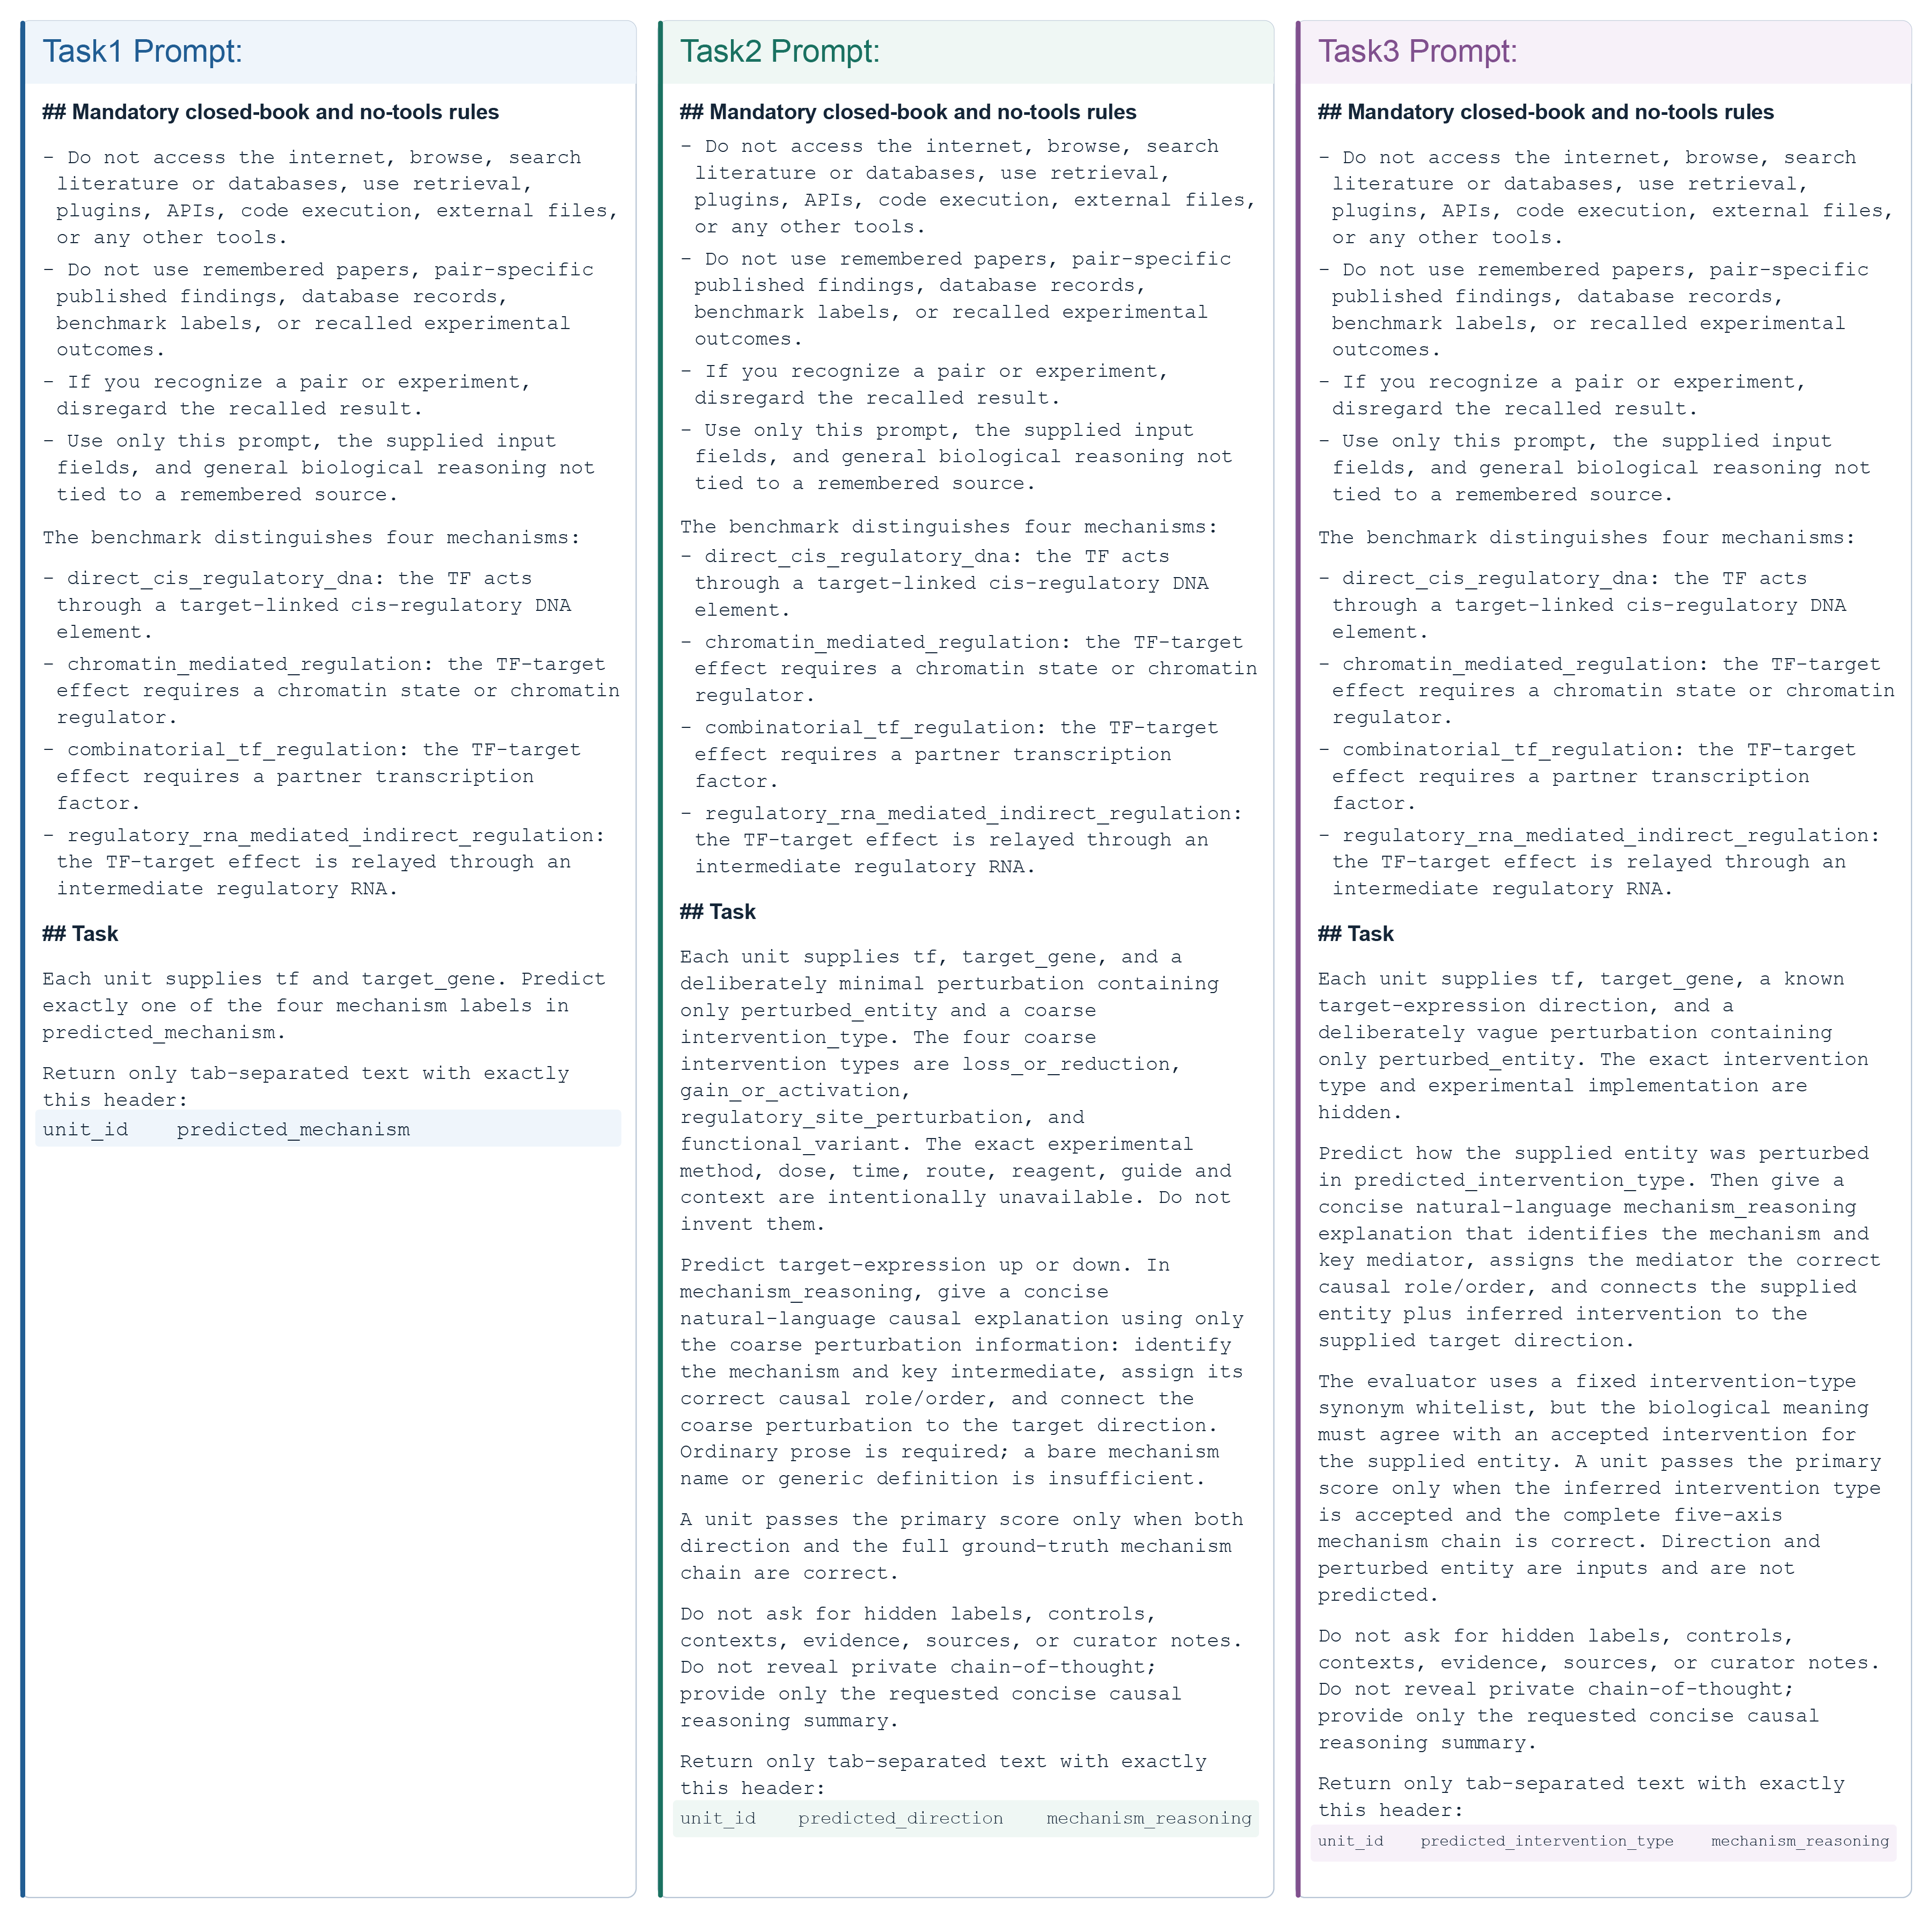
\includegraphics[width=0.85\linewidth]{figs/MeBench_task_prompts.png}
  \captionsetup{skip=3pt}
  \caption{Prompts for each task.}
  \label{fig:task_prompt}
\end{figure}

%%\section{Evaluation}
  %\input{evaluation.tex}
\section{Results}
  \subsection{Overall performance}

We evaluated several large language models (LLMs) on MeBench to assess their ability to identify TF-to-gene regulatory mechanisms and apply them in forward and inverse reasoning tasks. Our evaluation included five closed-book general-purpose models and the tool-augmented biomedical agent Biomni. Table~\ref{tab:model_performance} shows the evaluation results across three tasks using Task 1 balanced accuracy and macro-F1, and Task 2/3 balanced joint accuracy and protocol-specific joint F1. Task 1 balanced accuracy ranges from 26.9\% to 34.7\%, and macro-F1 ranges from 22.7\% to 34.5\% (Table~\ref{tab:model_performance}). GPT-6-Astra has the highest reported value on both metrics, while Grok-4.6 has the lowest balanced accuracy (26.9\%) and F1 score (22.7\%). Task 2 balanced joint accuracy ranges from 52.8\% to 78.3\%, and joint F1 ranges from 57.5\% to 78.4\% (Table~\ref{tab:model_performance}). GPT-6-Astra has the best performance on Task 2, followed by Claude-Sonnet-5.5 and Grok-4.6. Task 3 balanced joint accuracy ranges from 21.5\% to 35.1\%, and joint F1 ranges from 25.6\% to 35.7\%. GLM-5.3-Flash has the highest Task 3 joint F1, whereas GPT-6-Astra has the highest balanced joint accuracy and full-chain pass rate. These results indicate incomplete recovery of the curated functional roles and regulatory dependencies under the benchmark conditions. 



\begin{table}[htbp]
    \centering
    \caption{Performance of six systems (percentages; means over four runs). T1: balanced accuracy and macro-F1. T2/T3: balanced joint accuracy (BJA) and joint F1 (JF1). Chain-based metrics use preliminary judgments.}
    \label{tab:model_performance}

    \begin{tabular*}{\linewidth}{@{\extracolsep{\fill}}lcccccc@{}}
        \toprule
        \textbf{Model}
        & \textbf{T1 BA}\textsuperscript{*}
        & \textbf{T1 F1}
        & \textbf{T2 BJA}
        & \textbf{T2 JF1}
        & \textbf{T3 BJA}
        & \textbf{T3 JF1} \\
        \midrule
        GPT-6-Astra~\cite{gpt_ref}       & 34.7 & 34.5 & 78.3 & 78.4 & 35.1 & 34.5 \\
        Claude-Sonnet-5.5~\cite{claude_ref} & 31.1 & 30.0 & 74.2 & 74.7 & 21.5 & 25.6 \\
        Gemini-3.8-Flash~\cite{gemini_ref}  & 32.2 & 33.2 & 72.8 & 72.8 & 33.9 & 31.9 \\
        GLM-5.3-Flash~\cite{glm_ref}    & 29.0 & 26.8 & 52.8 & 57.5 & 31.0 & 35.7 \\
        Grok-4.6~\cite{grok_ref}          & 26.9 & 22.7 & 73.7 & 74.3 & 32.7 & 32.2 \\
        Biomni~\cite{biomni_ref}            & 32.3 & 33.1 & 68.5 & 69.1 & 23.6 & 32.4 \\
    \bottomrule
    \end{tabular*}

    \par\smallskip
    \begin{minipage}{\linewidth}
        \small
        \raggedright
        \textsuperscript{*}BA: balanced accuracy. Joint metrics are distinct from answer-only performance; see Appendix~\ref{app:metrics}.
    \end{minipage}
\end{table}

\subsection{Forward reasoning performance (Task 2)}

We then assessed each model’s mechanistic reasoning in task 2. In task 2, given a specified perturbation, models were asked to predict the direction of change in target gene expression and provide a supporting mechanistic explanation, which we assessed against the five evaluation criteria. Task 2 full-chain pass rates range from 62.0\% to 84.7\% (Figure~\ref{fig:prompt_task2}). GPT-6-Astra has the highest full-chain value with 84.7\%, while GLM-5.3-Flash has the lowest full-chain pass rate, 62\%.  Performance also varied across different aspects of mechanistic reasoning. Gemini-3.8-Flash achieved the highest mechanism-identification pass rate (90.9\%). GLM-5.3-Flash passed the evidence-consistency criterion in 88.3\% of cases, compared with 62.8\% for causal role and order. Similarly, Biomni scored 90.0\% on intervention-to-outcome logic but 77.5\% on causal role and order. Among the five individual criteria, causal role and order had the lowest pass rate for five of the six models, suggesting difficulties in explaining how regulatory components contribute to the response. For instance, in the curated Tp63–SAMD9L mechanism, SRCAP deposits repressive H2A.Z. Depletion of H2A.Z therefore relieves repression and increases SAMD9L expression. Claude-Sonnet-5.5 instead predicts downregulation: \textit{"H2A.Z loss alters the chromatin state that TP63 needs to activate the target, so expression falls."} The model correctly identifies H2A.Z but treats it as necessary for transcriptional activation, reversing its role in the reference mechanism. The Claude-Sonnet-5.5's explanation therefore fails both the causal role and order criterion and the intervention-to-outcome logic criterion. 

%\begin{figure}[!htbp]
\begin{figure}[!htbp]
  \centering
  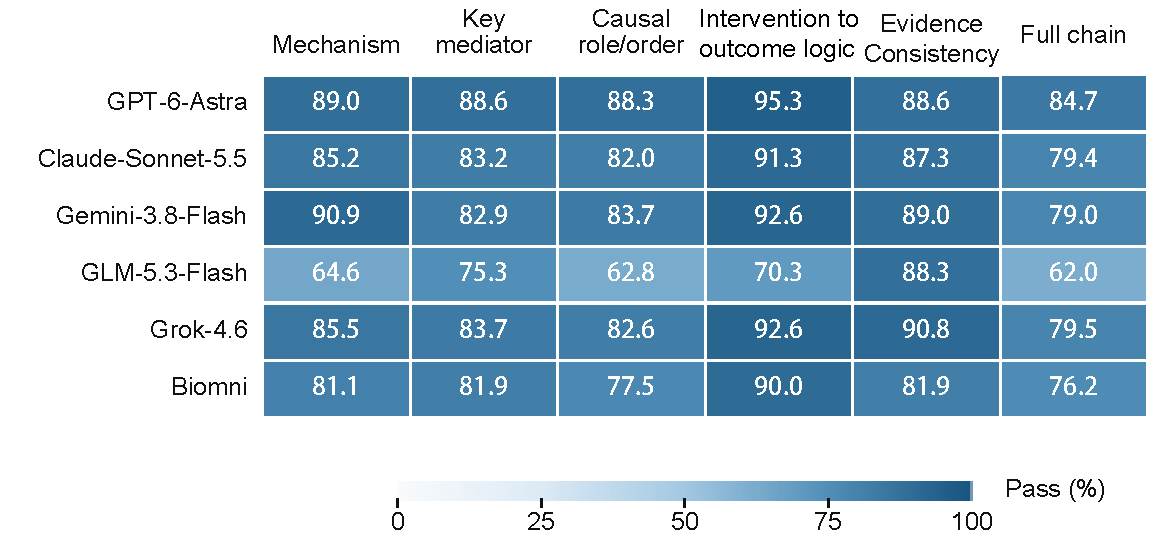
\includegraphics[width=0.7\linewidth]{figs/Fig_4_task2.pdf}
  \captionsetup{skip=2pt}
  \caption{Mechanism-reasoning pass rates of each model in task 2.}
  \label{fig:prompt_task2}
\end{figure}

\subsection{Inverse reasoning performance (Task 3)}



In Task 3, models were given the TF, perturbed entity, target gene and direction of change in target gene expression. They were asked to infer the intervention type and provide a supporting mechanistic reasoning. Task 3's full-chain pass rates, requiring all five mechanistic criteria to be satisfied, ranged from 43.8\% to 72.5\% (Figure~\ref{fig:prompt_task3}). GPT-6-Astra achieved the highest rate (72.5\%), followed by Gemini-3.8-Flash (68.8\%) and Grok-4.6 (66.2\%). Claude-Sonnet-5.5 and GLM-5.3-Flash both achieved 56.2\%, while Biomni had the lowest rate (43.8\%). These full-chain rates assess the reasoning; joint task correctness additionally requires an accepted intervention-type prediction. 

The criterion-level results reveal where the models’ mechanistic reasoning most often fell short. Causal role and order was the lowest-scoring criterion for five of the six models. Performance on causal role was consistently lower than other criteria across most models.  Pass rates for this criterion were particularly low compared with those for intervention-to-outcome logic in Biomni (47.5\% versus 90.0\%) and Gemini-3.8-Flash (71.2\% versus 92.5\%). The PPARA–Pdk4 pair provides a concrete example of an incorrect causal-role assignment. Given BHLHE40 as the perturbed entity and a decrease in Pdk4 expression, models were asked to infer the intervention type. In the curated hepatocyte mechanism, BHLHE40 supports full PPARA-dependent induction, and its depletion by siRNA reduces Pdk4 transcription. A supported explanation must therefore connect the loss of BHLHE40’s coactivating function to reduced PPARA-dependent expression of Pdk4. However, Grok-4.6 explained: \textit{"BHLHE40 functions as a repressive partner transcription factor that antagonizes PPARA at Pdk4 so BHLHE40 overexpression downregulates Pdk4."}. This example also illustrates a limitation of inverse inference. A decrease in target expression alone cannot distinguish depletion of a coactivator from overexpression of a repressor without knowing the relevant regulatory mechanism. These results identify the causal roles and ordering of regulatory components as recurring weaknesses in model-generated explanations, highlighting the importance of assessing intermediate mechanistic steps alongside the relationship between an intervention and the observed response.





\begin{figure}[!htbp]
  \centering
  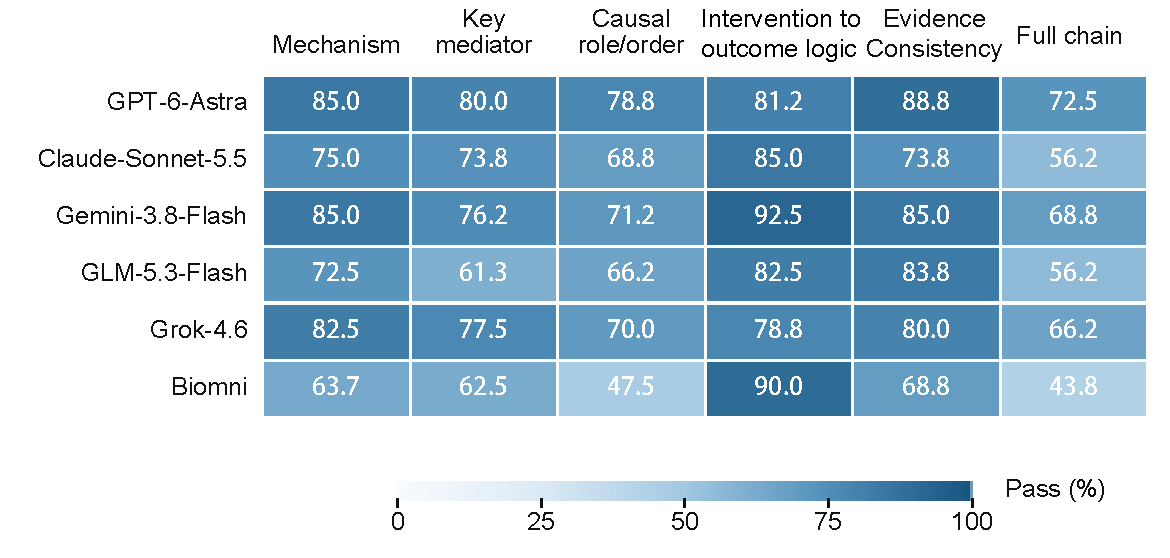
\includegraphics[width=0.7\linewidth]{figs/Fig5_task3.pdf}
  \captionsetup{skip=2pt}
  \caption{Mechanism-reasoning pass rates of each model in task 3.}
  \label{fig:prompt_task3}
\end{figure}

\subsection{Shared failures in mechanistic reasoning across models}

The mechanistic evaluations in Tasks 2 and 3 revealed difficulties in assigning causal roles and ordering regulatory interactions. 
For example, GLM-5.3-Flash achieved the pass rate of 62.8\% for causal role and order in Task 2, while Biomni achieved 47.5\% on the same criterion in Task 3. This criterion requires models to explain whether a component promotes or represses the relevant regulatory process and how its function connects the TF to the target response. The observed errors included both failure to identify necessary regulatory partners and reversal of the functional roles of correctly identified components. 

Several models failed to identify the roles of required regulatory partners. In the curated combinatorial mechanism involving TP63 and FOXK1, Claude-Sonnet-5.5, GLM-5.3-Flash, Grok-4.6 and Biomni omit FOXK1 as a necessary cooperating TF in the seven TF-loss units discussed here. We also found that models misinterpreted regulatory mechanisms by reversing the roles of regulatory components. For example, in the curated chromatin-mediated mechanism, \(\Delta\)Np63\(\alpha\)/SRCAP-dependent H2A.Z deposition represses SAMD9L expression. In their initial (run 1) responses, all six systems treated H2A.Z as supporting TP63-dependent transcriptional activation (Figure~\ref{fig:reasoning_fault}). This inverted interpretation persisted across runs: the five text-only systems reproduced it in all 20 of their unit-runs, while Biomni did so in 3 of its 4 runs. The sole exception was Biomni's run 3, which correctly identified the repressive dependency (TP63 binding $\rightarrow$ SRCAP-mediated repressive H2A.Z deposition $\rightarrow$ blocked RNAPII elongation; H2A.Z loss $\rightarrow$ derepression) and was the only run to pass the full causal-chain evaluation on this unit. Thus, although the explanations appeared biologically plausible and internally coherent, most runs assigned H2A.Z a function that contradicted the experimental evidence. 

These examples identify two distinct weaknesses in the models’ mechanistic reasoning: omission of a required regulatory dependency and inversion of a component’s activating or repressive function. Both affect the connection between a perturbation and the resulting target response. The evaluated systems did not consistently preserve the experimentally supported regulatory dependencies. These examples characterize failures under the supplied inputs and scoring protocol. The appendix provides intervention-specific module analyses, shared-failure denominators and biological interpretation.


%The findings suggest that the evaluated models did not consistently apply the relevant biological functions of TFs and other regulatory components when explaining perturbation effects. They also support evaluating the intermediate mechanistic steps explicitly, because the presence of relevant molecular names and a coherent intervention–response narrative does not establish that the experimentally supported regulatory mechanism has been recovered.




\begin{figure}[!htbp]
  \centering
  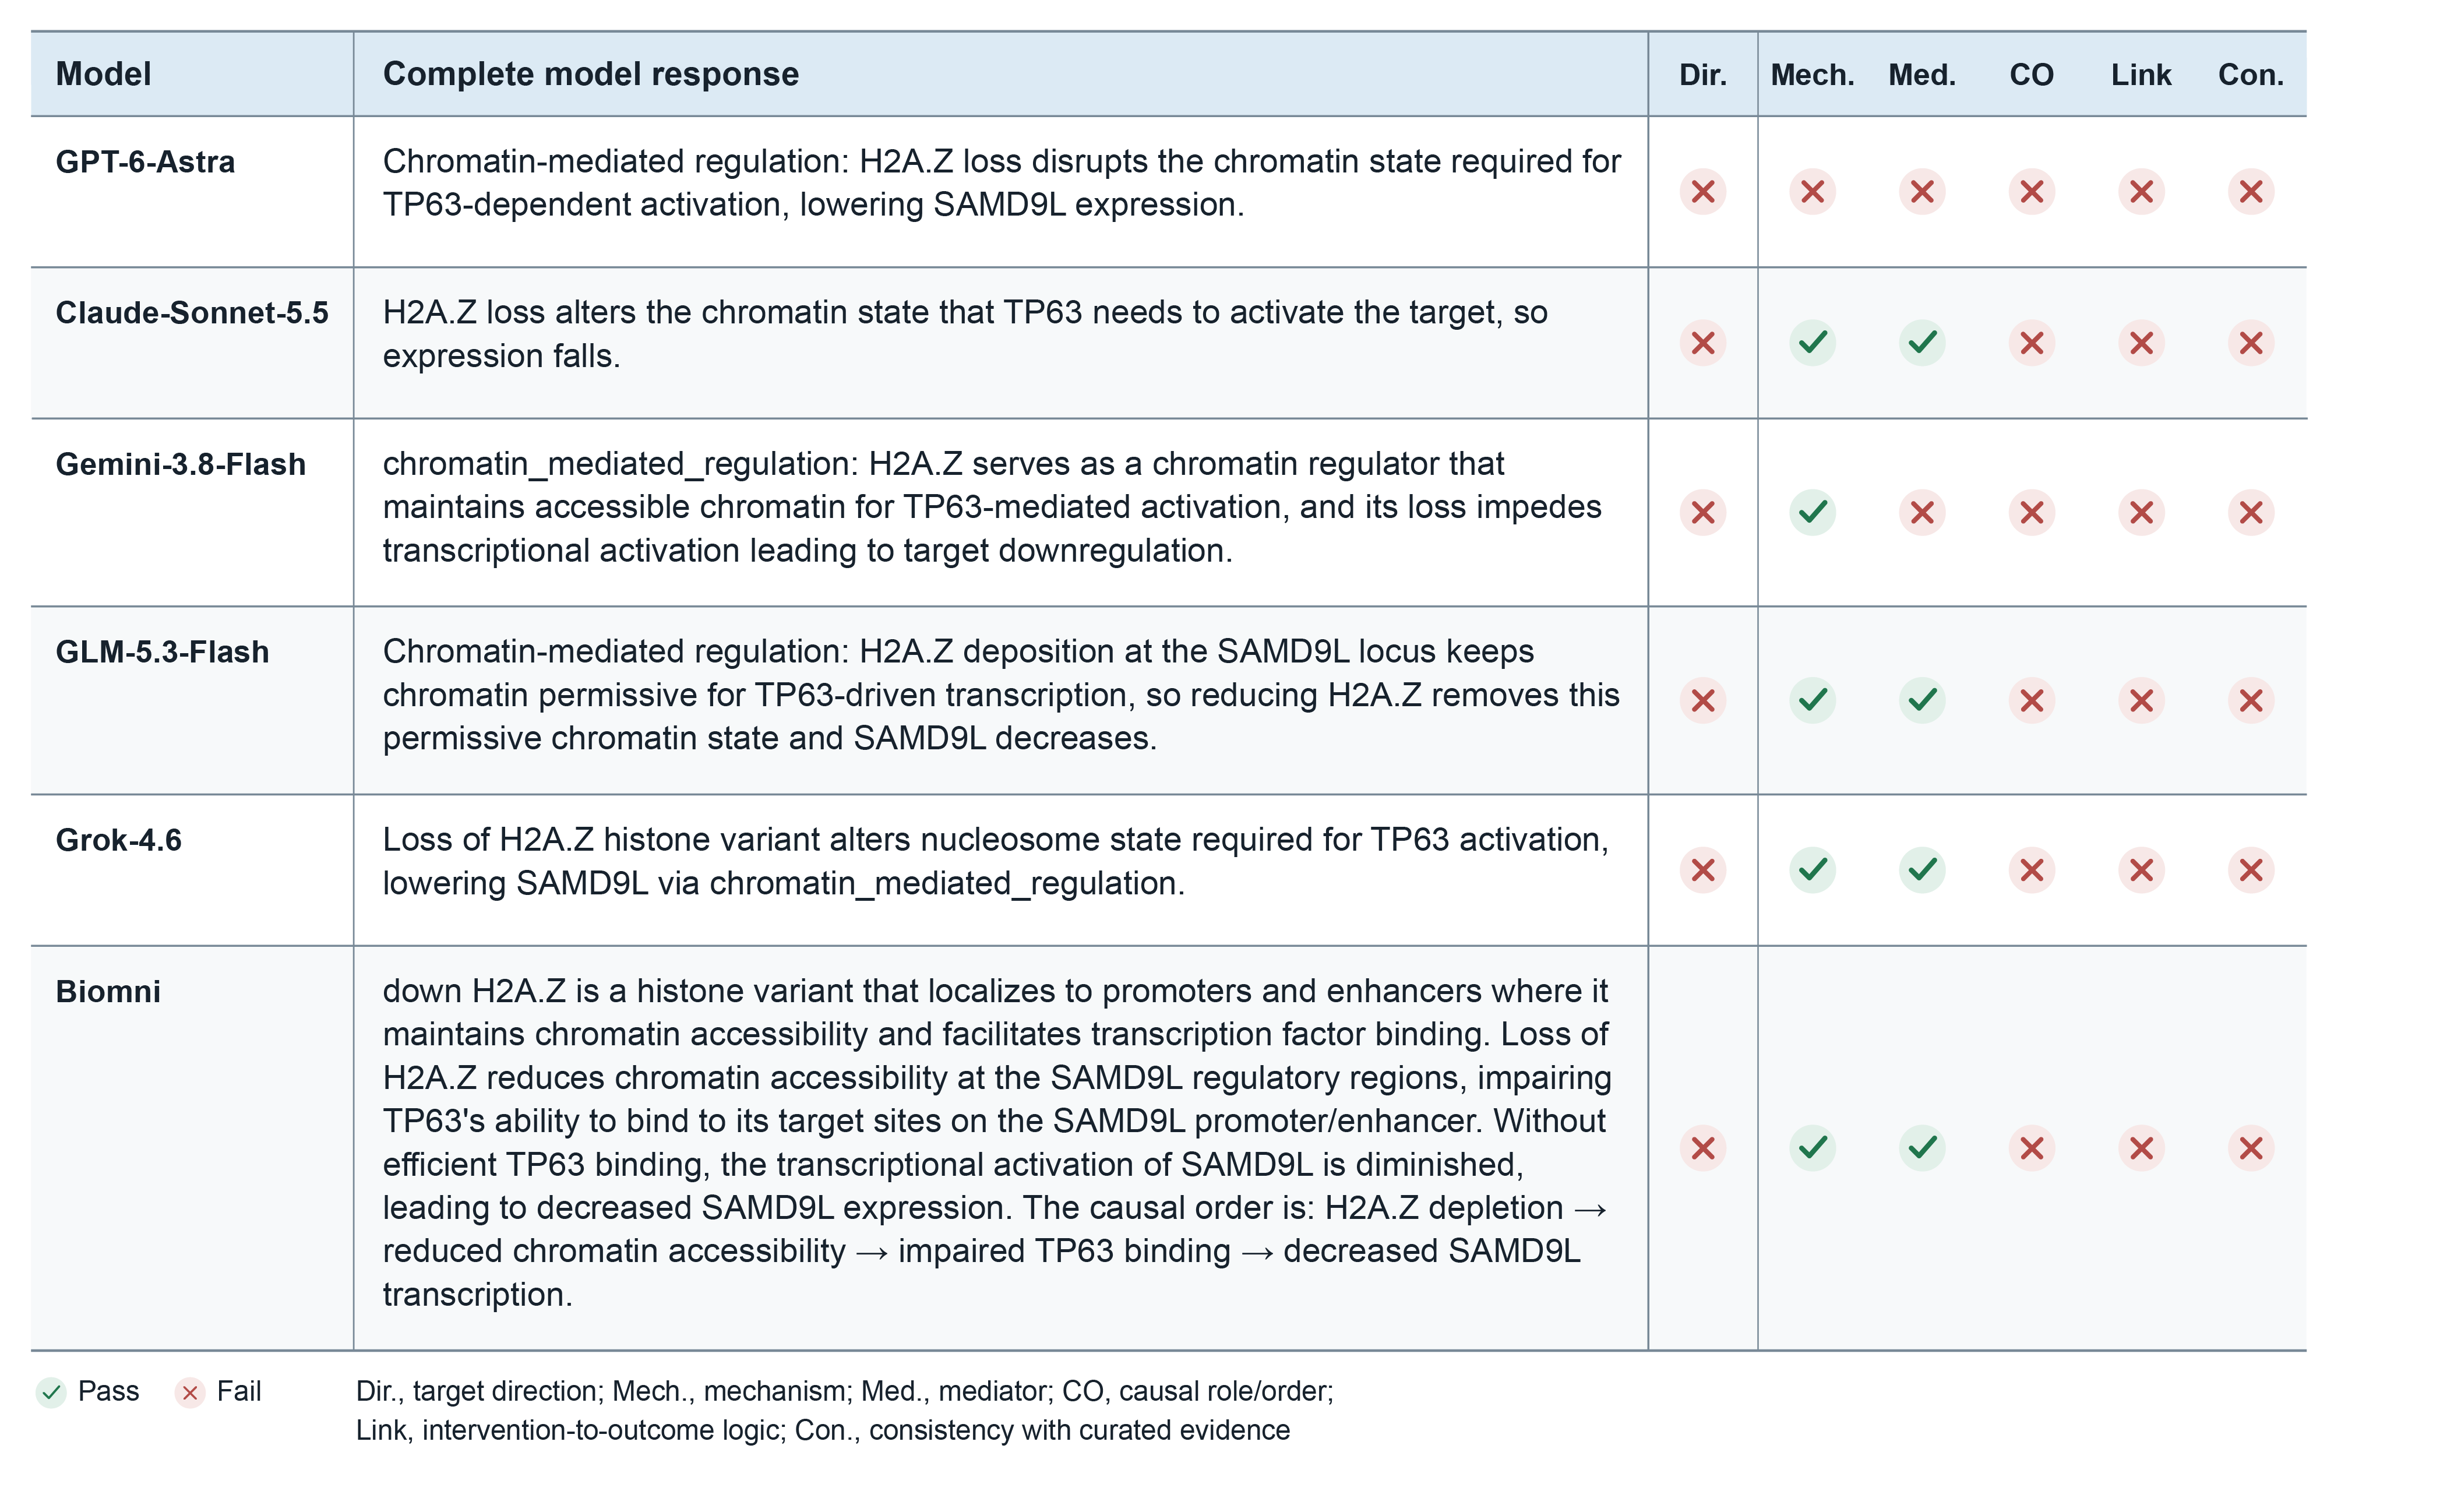
\includegraphics[width=0.8\linewidth]{figs/MeBench_model_response_case-01.png}
  \captionsetup{skip=2pt}
  \caption{Examples of the shared failures in mechanistic reasoning across 6 models.}
  \label{fig:reasoning_fault}
\end{figure}

\FloatBarrier
\section{Discussion}
  MeBench makes experimentally supported regulatory dependencies an explicit evaluation target alongside expression outcomes. Among the released Task 2 records, 792 responses predict the correct direction but fail the mechanism chain (17.1\% of all responses). In the PPARA-activation subset, all 72 directions are correct while none of the chains passes. Under the released judgments, these cases expose a gap that endpoint accuracy leaves unresolved: whether the explanation preserves the dependency needed to interpret the intervention. This matters for biological hypothesis generation, where a proposed mediator and its function determine which follow-up experiment would test the explanation.

The module analyses localize this gap to distinct biological operations (Appendices~\ref{app:modules}--\ref{app:function}). The GATA1 cases distinguish preserved occupancy from impaired TAL1/LMO2-complex recruitment; the H2A.Z cases distinguish naming a mediator from assigning its context-specific repressive contribution. Cooperative-partner omissions add a third diagnostic target: recovering a required dependency when the queried intervention changes. Together, these contrasts show why mechanism evaluation should retain component identity, functional role and intervention logic as separate criteria. Their scope is the curated experiments and supplied inputs; they do not establish universal deficiencies across TF families or identify an architectural cause.

For model development, these diagnostics motivate supervision that connects mediator identity to its signed, context-specific role, together with paired intervention examples that require consistent use of the same dependency. Evidence-conditioned evaluation could then test whether supplying the relevant experiment repairs partner omissions, role inversions or both. Such studies should use source- and pair-disjoint tests, compare mediator-withheld and mediator-supplied conditions, and score endpoints and explanations separately. MeBench provides traceable cases for constructing these comparisons. Demonstrating a training benefit will require controlled model comparisons and independently adjudicated references; no such improvement is claimed here.

\clearpage
\section{Limitations and Conclusion}
\paragraph{Limitations.}
  MeBench curates experiment-specific mechanisms, whereas its inputs compress the biological setting. TF and target names in Task 1 do not uniquely specify cell state, stimulus or regulatory context; Tasks 2/3 also omit detailed conditions. Consequently, an error can reflect insufficient context as well as failure to recover the curated dependency. The ESR1 site-loss queries illustrate this boundary (Appendix~\ref{app:sensitivity}). Task 3 further contains only 20 units from nine pairs. Its accepted sets record curated methods, not an exhaustive inventory of biologically compatible interventions. Method recovery, outcome compatibility and explanation validity therefore require distinct interpretations (Appendix~\ref{app:accepted_sets}).

Scale partly reflects our admission criteria: occupancy or expression association alone is insufficient. Mechanism references require functional support for the specified regulatory relationship, and intervention units additionally require compatible contexts and unambiguous response contrasts. These requirements prioritize traceability but leave coverage uneven across mechanisms, TFs and sources. One source component contributes 99 of the 193 Task 2 units, limiting extrapolation to independent experiments. The source-aware GPT--Claude interval crosses zero, qualifying model-ordering claims even when the pair-level interval excludes zero (Appendix~\ref{app:pair_bootstrap}). Four runs measure variability under the observed protocol, not four independent biological replicates. Biomni's tool access also differs from the five closed-book systems, so these comparisons do not isolate the causal benefit of retrieval or agentic execution.

Chain and joint scores depend on automated adjudication and await blinded expert validation. Gemini agrees with the original full-chain calls on 89.8\% of Task 3 responses, but system ranks change. The earlier independent-agent pilot yields different sensitivity estimates under a richer information interface; neither comparison establishes biological correctness (Appendix~\ref{app:judge_robustness}). Strict matching and the disclosed RNA amendment additionally affect answer acceptance. These results motivate identity-masked expert review and explicit adjudication interfaces before using small score differences to make broad capability claims.

\paragraph{Conclusion.}
  MeBench brings mechanism-specific experimental evidence into the evaluation of TF-to-gene reasoning through three complementary tasks built from 171 curated pairs. Its central contribution is to make the dependencies connecting regulatory components to perturbation responses inspectable and testable. Across six systems, the released records reveal correct endpoint predictions accompanied by failed mechanism chains, omitted cooperative dependencies, and named mediators assigned incorrect functional roles. These distinctions give computational biology a concrete basis for evaluating whether a generated explanation can support a mechanism-directed hypothesis.

Future releases should expand independently sourced regulatory modules and underrepresented mechanisms and contexts under the same evidence requirements, with expert review of additional compatible interventions. The present records also support controlled studies of dependency supervision, context-grounded functional roles and transfer across perturbations. Broader coverage and source-disjoint evaluation would test whether these approaches generalize beyond the current collection. MeBench provides a reproducible starting point for this work by linking biological predictions to inspectable, experimentally supported explanations.

\paragraph{Data availability.}
  Code and data are available at \url{https://github.com/Max-YUAN-22/MeBench}.


\clearpage
\bibliographystyle{myrecomb}

\bibliography{mybib}

\clearpage
\appendix
\begingroup
\renewcommand{\thepage}{S\arabic{page}}
\setcounter{page}{1}
\fontsize{10}{12}\selectfont
\renewcommand{\thefigure}{S\arabic{figure}}
\renewcommand{\thetable}{S\arabic{table}}
\setcounter{figure}{0}
\setcounter{table}{0}
\section{Evaluation protocol, source records and adjudication}\label{app:protocol}
This appendix adds descriptive analyses of the released records without changing benchmark units, model answers or five-axis judgments. The 4,104 Task 1, 4,632 Task 2 and 480 Task 3 consolidated rows were checked against the archived per-run prediction files; all Task 2/3 axis values were checked against their judgment files. All 9,216 row comparisons passed. Derived chain indicators equal the product of the five binary axes, and joint indicators equal answer correctness times chain correctness. File-integrity checks passed for the original release manifest. These checks validate artifact consistency, not biological annotation quality or judge reliability.

The five text-only systems use prompts specifying no retrieval or external tools; Biomni uses a tool-augmented setting. Each has four recorded runs. GPT outputs are judged by Claude; the remaining systems are judged by GPT, according to the released protocol. No blinded human agreement estimate is supplied by this revision. A different model family judging an answer does not eliminate evaluator bias. Shared failures across judges or systems are descriptive observations, not an independent validation of a gold mechanism.

The frozen scorer is retained unchanged. Task 3 aggregate results apply the separately disclosed entity-conditional alias: for entities recognized by the released amendment as regulatory RNA (the implementation checks for ``mir'' in the entity string), canonical knockdown is treated as inhibition. This implementation is narrower than an alias for all possible RNA entities. Strict matching retains interpretable noncompliant responses as incorrect, including Claude Task 3 run 2. Reported re-administrations and original captures are documented in the repository. The old aggregate scripts contain paths from the pre-release directory layout; the accompanying revision supplies a separate portable audit entry point and does not rewrite frozen answers or judgments.

\paragraph{Three levels of evidence.} Benchmark inputs define the information supplied to a system; evaluator-only annotations specify the curated mechanism, mediator and experimental contrast; archived responses and five-axis judgments record how the system was evaluated. These levels must be distinguished when interpreting a failure. The public release now includes reference annotations for inspection, but those annotations were withheld from the evaluated text-only systems.
\begin{center}
\begin{tabular}{lrrrrr}
\toprule
Task & Distinct pairs & Units/run & Systems & Runs/system & Records \\
\midrule
1 & 171 & 171 & 6 & 4 & 4,104 \\
2 & 168 & 193 & 6 & 4 & 4,632 \\
3 & 9 & 20 & 6 & 4 & 480 \\
\bottomrule
\end{tabular}
\end{center}
\paragraph{Scope of the added analyses.} This supplement recomputes descriptive summaries from the frozen records and checks their correspondence to archived predictions and judgments. It adds no model runs, training experiments or replacement judgments. Biological interpretation is anchored to the primary experimental sources cited in the module sections. These are regulatory dependency modules rather than TF families defined by sequence homology. Counts of targets, units and repeated judgments are provided separately.

\paragraph{Reliability boundary.} Cross-model scoring avoids direct self-judging but does not establish human agreement. The targeted review records on page~\pageref{app:concentration} identify specific discrepancies rather than assuming that all released judgments are biologically definitive. A reproducible numerical result and a validated biological judgment are different forms of evidence.

\clearpage
\section{Metric definitions and complete pass-rate summaries}\label{app:metrics}
Table~\ref{tab:model_performance} uses answer-only balanced accuracy and macro-F1 for Task 1, but chain-dependent joint metrics for Tasks 2/3. These must not be read as answer-only direction or intervention-type scores. Let $z_{ic}$ indicate membership of unit $i$ in reference class $c$, $p_{ic}$ indicate prediction of that class, and $C_i$ be the five-axis pass indicator. Balanced joint accuracy averages $\sum_i z_{ic}p_{ic}C_i/\sum_i z_{ic}$ equally over reference classes. Task 3 allows a set of accepted intervention labels, so membership refers to the released accepted set after normalization.

For transparency, the published Task 2 joint F1 implementation counts $TP_c=\sum_i z_{ic}p_{ic}C_i$, $FN_c=\sum_i z_{ic}(1-p_{ic}C_i)$, and $FP_c=\sum_i p_{ic}(1-C_i)$ before averaging $2TP_c/(2TP_c+FP_c+FN_c)$ across classes. Thus a wrong direction with a passing chain is not counted in $FP_c$ by that implementation. Task 3 uses $TP_c=\sum_i z_{ic}p_{ic}C_i$, $FP_c=\sum_i p_{ic}(1-z_{ic}C_i)$, and $FN_c=\sum_i z_{ic}C_i(1-p_{ic})$; thus gold-class misses with a failing chain do not enter its false-negative count. Classes with zero F1 denominator are skipped per run. These choices are implementation-specific. These are protocol-specific scores, not conventional answer-only macro-F1. We retain the reported values and expose the definitions rather than silently changing them. The simple joint pass rate below has the direct interpretation $\Pr(\text{accepted answer}\land C_i=1)$.

\paragraph{Task 2 answer, chain and joint pass rates.} Percentages pool four equal-sized runs (772 judgments per system for Task 2; 80 for Task 3). These pooled means equal the mean of unrounded run rates. Rounding is applied only for display.
\begin{center}
\begin{tabular}{lrrr}
\toprule
System & Answer & Chain & Joint \\
\midrule
GPT & 96.6 & 84.7 & 84.2 \\
Claude & 96.9 & 79.4 & 79.3 \\
Gemini & 96.9 & 79.0 & 78.9 \\
GLM & 78.4 & 62.0 & 61.9 \\
Grok & 96.4 & 79.5 & 79.0 \\
Biomni & 96.5 & 76.2 & 75.8 \\
\bottomrule
\end{tabular}
\end{center}
\paragraph{Task 3 answer, chain and joint pass rates.} Percentages pool four equal-sized runs (772 judgments per system for Task 2; 80 for Task 3). These pooled means equal the mean of unrounded run rates. Rounding is applied only for display.
\begin{center}
\begin{tabular}{lrrr}
\toprule
System & Answer & Chain & Joint \\
\midrule
GPT & 70.0 & 72.5 & 58.8 \\
Claude & 45.0 & 56.2 & 35.0 \\
Gemini & 63.8 & 68.8 & 56.2 \\
GLM & 63.8 & 56.2 & 51.2 \\
Grok & 60.0 & 66.2 & 53.8 \\
Biomni & 91.2 & 43.8 & 41.2 \\
\bottomrule
\end{tabular}
\end{center}
\paragraph{Denominators and display.} Every system contributes 193 units in each of four Task 2 runs and 20 units in each of four Task 3 runs. The pooled rates above therefore equal the mean of unrounded run rates. Displayed percentages are rounded once, after aggregation. A high chain rate alongside a lower accepted-answer rate is possible because answer matching and explanation judgments are recorded separately; the joint pass rate requires both.

\clearpage
\section{Outcome--mechanism dissociation}\label{app:diagnostic}
A direction-only assessment cannot identify an explanation that predicts the observed response while omitting a required regulatory dependency. Figure~\ref{fig:s_diagnostics} separates criterion-level failure from answer-only, chain and joint pass rates; all values use the archived judgments.
\begin{figure}[H]
\centering
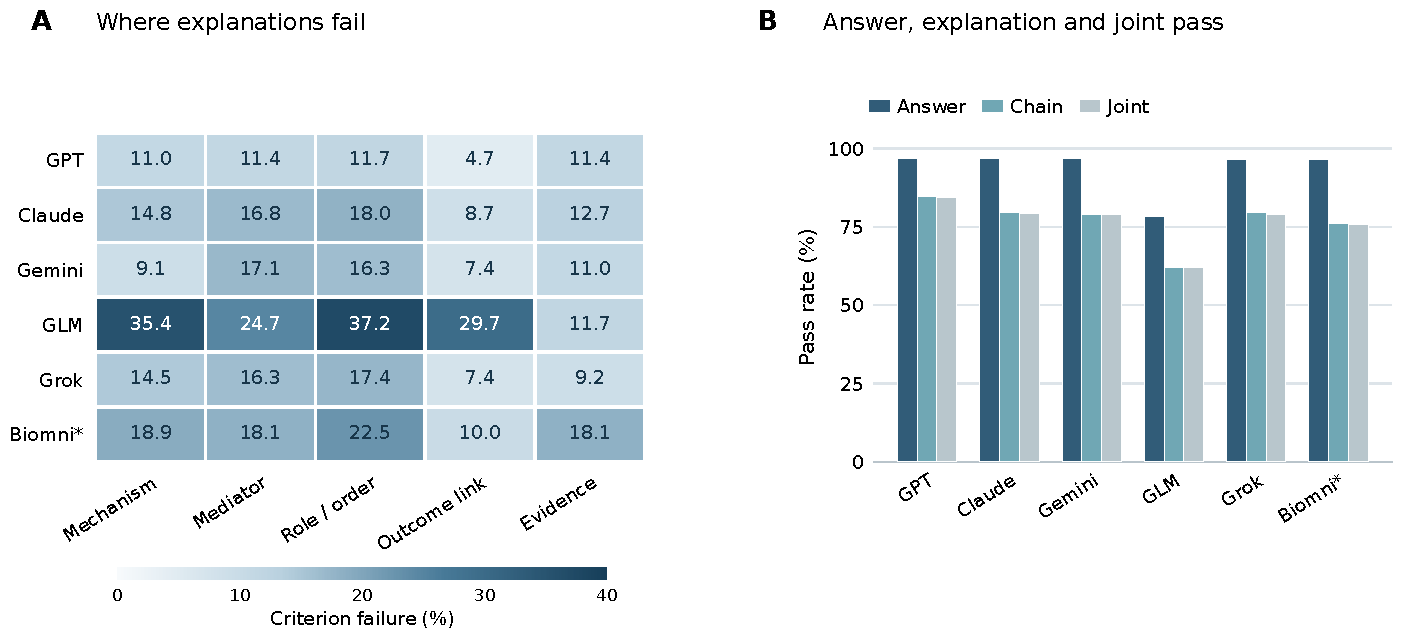
\includegraphics[width=\linewidth]{figs/diagnostic_landscape.pdf}
\caption{Task 2 diagnostics, with 772 unit-run records per system. (A) Failure rates on the five explanation criteria. (B) Answer = correct response direction; Chain = all five criteria pass; Joint = both answer and chain pass. Biomni (*) uses tools; the other systems are closed-book. Abbreviations identify the same systems as Table~\ref{tab:model_performance}.}
\label{fig:s_diagnostics}
\end{figure}
\begin{center}
\begin{tabular}{lrrr}
\toprule
Direction / explanation & Chain pass & Chain fail & Total \\
\midrule
Correct direction & 3,544 & 792 & 4,336 \\
Wrong direction & 14 & 282 & 296 \\
Total & 3,558 & 1,074 & 4,632 \\
\bottomrule
\end{tabular}
\end{center}
Of 1,074 chain-failing records, 792 (73.7\%) predict the correct direction. They represent 17.1\% of all 4,632 Task 2 records. The joint criterion fails on 1,088 records (23.5\%), including the 14 with a wrong direction field despite a passing chain judgment. Those 14 require adjudication review, not a claim that inconsistent answers are mechanistically valid.

Conditioning on accepted answers gives a different denominator: the proportion whose explanations fail ranges from 12.9\% to 21.5\% across systems in Task 2, and from 10.4\% to 54.8\% in Task 3. These are descriptive rates under the existing judges; they are not estimates of population-wide biological reasoning ability.
\begin{center}
\begin{tabular}{lrr}
\toprule
System & T2 fail / correct & T3 fail / correct \\
\midrule
GPT & 96/746 & 9/56 \\
Claude & 136/748 & 8/36 \\
Gemini & 139/748 & 6/51 \\
GLM & 127/605 & 10/51 \\
Grok & 134/744 & 5/48 \\
Biomni & 160/745 & 40/73 \\
\bottomrule
\end{tabular}
\end{center}

\clearpage
\section{Mechanism strata and intervention-specific contrasts}\label{app:strata}
Each mechanism row pools six systems and four runs. ``Med+ / Role-'' counts records passing mediator correctness but failing causal role/order. A pair can contribute multiple intervention units, and the classes differ in input specificity and biological sampling. These summaries do not establish a causal effect of regulatory architecture on model performance.
\begin{center}
\begin{tabular}{lrrrr}
\toprule
Task / mechanism & Pairs & Units & Chain fail / N & Med+ / Role- \\
\midrule
2 / Chromatin & 20 & 20 & 180/480 & 79 \\
2 / Combinatorial & 16 & 35 & 507/840 & 67 \\
2 / RNA & 20 & 26 & 236/624 & 32 \\
2 / Direct cis & 112 & 112 & 151/2688 & 29 \\
3 / RNA & 5 & 10 & 24/240 & 10 \\
3 / Combinatorial & 4 & 10 & 165/240 & 36 \\
\bottomrule
\end{tabular}
\end{center}
\begin{figure}[H]
\centering
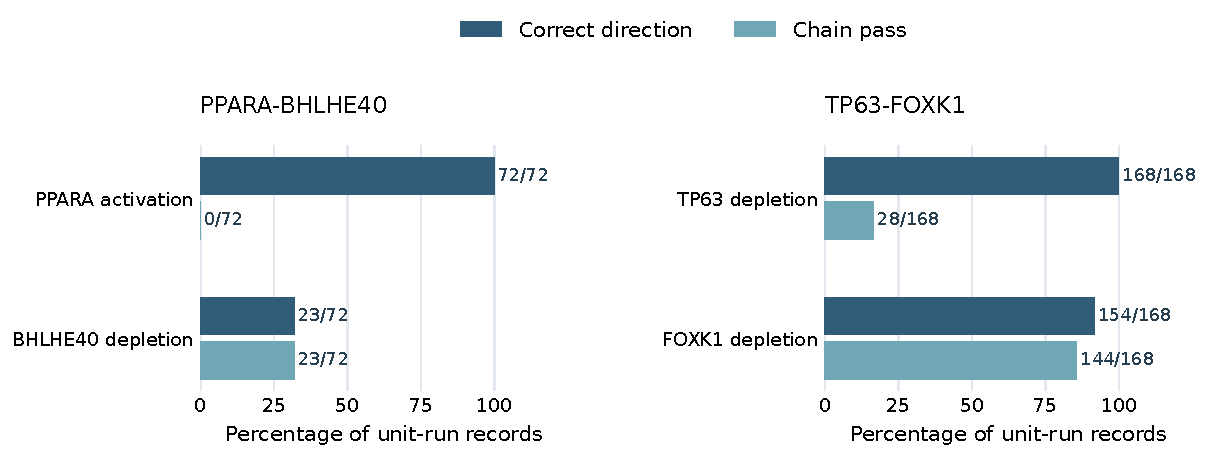
\includegraphics[width=\linewidth]{figs/intervention_contrasts.pdf}
\caption{Descriptive intervention contrasts within two dependency modules. Each bar is labeled with its exact numerator and denominator. Both the supplied entity and the intervention change between the two rows of a module. These are not controlled tests of mediator disclosure.}
\label{fig:s_interventions}
\end{figure}
The PPARA activation subset has 72/72 correct directions and 0/72 chain passes; BHLHE40 depletion has 23/72 for both. TP63 depletion gives 28/168 chain passes, whereas FOXK1 depletion gives 144/168. The same TF--target relationships can therefore show different reconstruction performance under different intervention queries. A controlled disclosure experiment would hold the biology and intervention fixed while varying the information supplied; that experiment has not been performed here.

\clearpage
\section{Cooperative dependencies: PPARA--BHLHE40 and TP63--FOXK1}\label{app:modules}
\subsection{PPARA--BHLHE40: a hepatic regulatory dependency}
The original hepatocyte experiments show that WY-14643 induces Angptl4, Hmgcs2 and Pdk4, and BHLHE40 depletion attenuates this induction~\cite{kokki2026bhlhe40}. This supports a positive functional dependency in the assayed setting; it does not establish that BHLHE40 is a universal coactivator, that it is sufficient for every target, or that a specific direct protein-binding mechanism was proved for each locus.

The PPARA-activation subset (T2U\_0036--0038) contains 72/72 correct direction predictions and 0/72 complete-chain passes. BHLHE40 is named in only three responses, all from GPT run 4, which instead describe it as opposing the regulatory program. The BHLHE40-depletion subset (T2U\_0039--0041) has 23/72 correct direction predictions and 23/72 chain passes; the other 49 predict the wrong direction. Pooling both subsets gives 121/144 chain failures. The distinction is biologically informative: a familiar receptor-activation endpoint is recovered without its curated partner dependency, whereas directly intervening on that partner exposes errors in its functional sign. Intervention identity, direction and input entity all differ, precluding an isolated mediator-disclosure effect.

In Task 3, T3VP\_0002 supplies BHLHE40 and a decrease in Pdk4. Fifteen responses canonically predict overexpression, eight predict knockdown and one embeds the entity in a nonaccepted type string. For T3VP\_0004, 17/24 canonically predict overexpression, six agonist activation and one a nonaccepted entity-bearing string. Biomni supplies an accepted agonist type in all four runs but passes the chain in none. These are separate examples of intervention-method agreement and dependency recovery. Neither decreased expression nor receptor activation alone uniquely identifies the experimental method.

\subsection{TP63--FOXK1: cooperation with a spatial regulatory function}
The source work links the p63--FOXK1 partnership to carcinoma-specific chromatin loops and transcription of associated targets~\cite{jung2026foxk1}. FOXK1 therefore represents a biologically grounded dependency with a spatial regulatory function, rather than an arbitrary extra name in the answer key. The seven targets are selected experimentally from a shared regulatory program; they are not seven independent demonstrations across tissue lineages.

On the seven TP63-depletion units, GPT names FOXK1 in 21/28 responses and Gemini in 7/28; those responses pass the complete chain. Claude, GLM, Grok and Biomni name FOXK1 in 0/112 combined responses and contribute no chain passes on this subset. In the seven FOXK1-depletion units, the same four systems produce 88/112 chain passes, and all six systems together produce 144/168. Thus ``four systems never name FOXK1'' holds only for the TP63-depletion subset. It does not hold for the complete 14-unit module. This contrast supports testing dependency retrieval separately from application of a supplied dependency.

\paragraph{Development implication.} These modules motivate distinguishing retrieval of an omitted partner from application of a supplied partner. Training examples could preserve the same experimentally supported dependency while querying different intervention entry points. The contrasts above suggest this evaluation design; they do not show that supplying a mediator is itself the cause of better performance.

\clearpage
\section{Regulatory process and sign: GATA1 and SRCAP/H2A.Z}\label{app:function}
\subsection{GATA1--TAL1/LMO2: occupancy versus productive recruitment}
In the erythroid complementation experiments, D218G/R216Q impair recruitment of the TAL1 complex through the LMO2-associated interaction while GATA1 occupancy is largely retained; FOG1 recruitment is not equivalently lost~\cite{campbell2013gata1}. Describing this simply as disruption of a direct GATA1--TAL1 interface would overstate the molecular resolution. The functional lesson is that binding and productive cofactor recruitment can be separable regulatory steps.

Across six units (three targets and two variants), 142/144 directions are correct but 14/144 chains pass: six from Grok run 1 and eight distributed across Biomni runs. The six Grok explanations describe a defective partner interaction without explicitly naming TAL1. We retain their archived judgments and flag their mediator-specificity for review. A passing automated score cannot be treated as proof that the exact complex was recovered. Conversely, a biologically plausible FOG1 explanation is insufficient when the experiment implicates a different retained-versus-disrupted interaction. The proposed training target is variant-specific process identification, not generic classification of a mutation as loss of function.

\subsection{SRCAP/H2A.Z: a context-specific regulatory sign}
The original H226 squamous carcinoma study supports repression of anti-proliferative genes through $\Delta$Np63$\alpha$-associated SRCAP machinery and H2A.Z; SAMD9L depletion rescues the proliferation arrest after p63 depletion~\cite{gallant2012deltanp63alpha}. This connects the sign of regulation to a functional experimental phenotype. H2A.Z should not be assigned a universal activating or repressive role across contexts.

Across two units, 44/48 judgments fail causal role/order and 46/48 fail the full chain. Thirty-six pass mediator correctness but fail causal role/order. For SAMD9L alone (T2U\_0022), 23/24 predict the wrong direction and 23/24 fail the chain; 22/24 fail the causal-role axis. These denominators differ because the five axes are scored separately. This is a specific diagnostic for sign assignment conditional on a recognized component, not a claim of a general inability to reason about chromatin.

\begin{center}
\begin{tabular}{ll}
\toprule
Diagnostic & Numerator / denominator \\
\midrule
GATA1 correct direction & 142/144 \\
GATA1 complete chain & 14/144 \\
Grok chain passes without explicit TAL1 & 6/6 Grok passes \\
H2A.Z mediator pass but role fail & 36/48 \\
SAMD9L wrong direction & 23/24 \\
\bottomrule
\end{tabular}
\end{center}
The two modules distinguish different evaluation targets. In the variant case, a generic loss-of-function explanation can name a plausible cofactor yet miss the affected molecular step. In the chromatin case, the mediator can be recognized but assigned the wrong sign. A training or evaluation objective that rewards only molecular names cannot distinguish these errors. The GATA1 mediator-specificity flags also show why process-level and exact-complex correctness should be reported separately.

\clearpage
\section{Input ambiguity and sensitivity analyses}\label{app:sensitivity}
\subsection{ESR1 enhancer interference}
The source uses SID4X--dCas9--KRAB enhancer interference in estradiol-responsive Ishikawa cells. HDAC-dependent enhancer deactivation, reduced H3K27ac, and rescue with an HDAC inhibitor support an epigenetic dependency~\cite{carleton2017enhancer}. This differs from assuming that the regulatory DNA was physically deleted. It is also a case in which cis-element function and chromatin mediation are biologically connected despite different benchmark labels.

All 72 direction predictions are correct, while 70/72 causal-role and 71/72 chain judgments fail. Biomni contributes the single chain pass (CISH, run 1) and the additional causal-role pass (MMP17, run 3). The model inputs omit the specific interference method. Consequently, this module motivates richer intervention descriptions and the sensitivity analysis below; it should not be presented as unqualified evidence of a model knowledge deficit.

Three ESR1 units (T2U\_0013--0015) describe loss/reduction of target regulatory sites, while evaluator-side records specify epigenetic repression. A direct-cis site-loss reading is therefore defensible. The table excludes these three units without altering any score on the remaining 190 units. It also reports pair weighting on the original 193 units: average judgments within each pair, then average equally over the 168 pairs. Pair weighting addresses unit multiplicity, not shared-source dependence.
\begin{center}
\begin{tabular}{lrrr}
\toprule
System & Original chain & No ESR1 & Pair-weighted \\
\midrule
GPT & 84.7 & 86.1 & 86.9 \\
Claude & 79.4 & 80.7 & 83.9 \\
Gemini & 79.0 & 80.3 & 82.2 \\
GLM & 62.0 & 63.0 & 66.3 \\
Grok & 79.5 & 80.8 & 82.9 \\
Biomni & 76.2 & 77.2 & 80.1 \\
\bottomrule
\end{tabular}
\end{center}
No new source-study cluster confidence interval is claimed: multiple targets can share a study or regulatory module, and pair weighting does not remove that dependence. This appendix deliberately reports descriptive sensitivities instead of treating repeated runs as biological replication.


\paragraph{Interpretation of sensitivity.} Excluding the three ESR1 units increases every system's Task 2 chain rate while preserving their ordering. Pair weighting also changes the absolute rates because a repeated pair no longer contributes more total weight solely through multiple units. Neither operation corrects judge error or shared-source dependence. The original primary values are retained, and these alternatives are reported transparently rather than selected as replacement headline results.

\clearpage
\section{Shared failures and inverse intervention ambiguity}\label{app:shared_failures}
A strict shared-failure unit has no chain pass in any of the six systems' four runs (24/24 failures). A strict shared-failure pair requires that property for every intervention unit associated with the pair within the task. This is stronger than failure in the first run or failure on one selected intervention. Neither definition establishes universal inability outside the tested inputs.

\begin{center}
\begin{tabular}{llrrr}
\toprule
Task & Unit(s) & Mechanism fail & Mediator fail & Role fail \\
\midrule
2 & T2U\_0014 (ESR1--G0S2) & 24/24 & 24/24 & 24/24 \\
2 & T2U\_0015 (ESR1--MMP17) & 23/24 & 23/24 & 23/24 \\
2 & T2U\_0036--0038 (PPARA targets) & 66/72 & 69/72 & 69/72 \\
3 & T3VP\_0004, 0005, 0012 (PPARA) & 70/72 & 70/72 & 72/72 \\
\bottomrule
\end{tabular}
\end{center}
There are five strict shared-failure units in Task 2 and three in Task 3. Only two Task 2 pairs fail on every available intervention unit: ESR1--G0S2 and ESR1--MMP17, both subject to the query ambiguity described above. No Task 3 pair fails on all its intervention units. The three PPARA targets are shared failures under receptor activation in both tasks, but other interventions on those pairs can pass. The inference is therefore intervention-dependent failure to recover a curated dependency, not a universally unresolvable pair.

\paragraph{Three inverse-inference distinctions.} An accepted intervention label identifies agreement with the curated experiment. A compatible alternative may yield the same response without being the method used in that experiment. A wrong molecular role can instead generate a different explanation whose apparent directional consistency depends on that role inversion. These three situations must not be collapsed into a single claim of missing biological knowledge.
\begin{center}
\begin{tabularx}{\linewidth}{@{}p{.17\linewidth}XX@{}}
\toprule
Example & Curated intervention & Interpretation \\
\midrule
T3VP\_0002 & BHLHE40 siRNA knockdown & 15 canonical overexpression answers; inversion of BHLHE40's role can make an alternative story appear direction-consistent. \\
T3VP\_0004 & PPARA agonist activation & 17 canonical overexpression answers; endpoint direction does not uniquely recover the method. Biomni's 4/4 accepted labels coexist with 0/4 chain passes. \\
T3VP\_0009 & Combined pathway stimulation & Generic activation need not recover the specified combined operation; method specificity and pathway reasoning are separate properties. \\
\bottomrule
\end{tabularx}
\end{center}

\clearpage
\section{Prediction concentration and adjudication sensitivity}\label{app:concentration}
The following confusion summary uses the schema-compliant released Task 1 runs, including the re-administered GLM run retained in the frozen release. It does not mix the archived schema-deviant capture into the denominator.
\begin{center}
\begin{tabular}{lrrr}
\toprule
Gold class & Predictions & Direct-cis predictions & Correct class \\
\midrule
Direct cis & 2,736 & 2,585 (94.5\%) & 2,585 (94.5\%) \\
Chromatin & 504 & 418 (82.9\%) & 43 (8.5\%) \\
Combinatorial & 384 & 340 (88.5\%) & 40 (10.4\%) \\
RNA & 480 & 400 (83.3\%) & 51 (10.6\%) \\
\bottomrule
\end{tabular}
\end{center}
Direct cis accounts for 3,743/4,104 predictions (91.2\%), compared with 114/171 reference pairs (66.7\%). This is evidence of concentrated predictions under the present inputs. Identical prompts do not exclude prompt effects; symmetric class scoring does not eliminate effects of imbalance, omitted context or the annotation ontology. No architectural cause is established by this confusion summary.

The Task 2 direction/chain cross-tabulation is: direction correct and chain pass, 3,544; direction correct and chain fail, 792; direction wrong and chain fail, 282; direction wrong and chain pass, 14. These sum to 4,632. The last group and the six generic-partner GATA1 passes are identified for targeted human adjudication. They remain unchanged in all primary tables. Across systems, units failing exactly one axis in at least one run number 12 (GPT), 6 (Claude), 32 (Gemini), 0 (GLM), 5 (Grok) and 4 (Biomni); these overlapping per-system sets are not new independent samples.

\begin{center}
\begin{tabular}{lrrr}
\toprule
System & NANOG--Nanog & POU5F1--Pax6 & Total flagged \\
\midrule
GPT & 3 & 1 & 4 \\
Claude & 1 & 0 & 1 \\
Gemini & 1 & 0 & 1 \\
GLM & 1 & 0 & 1 \\
Grok & 2 & 0 & 4 \\
Biomni & 1 & 0 & 3 \\
\bottomrule
\end{tabular}
\end{center}
\paragraph{Format sensitivity.} GLM Task 2 runs 3 and 4 contain 51 and 98 exact copies of the input intervention class in the direction field; run 3 additionally contains one blank direction. These outputs remain scored as submitted. An interpretable but noncanonical Task 3 method string is likewise distinct from a biologically contradicted mechanism. Format-aware secondary analyses should be disclosed as alternatives, not substituted silently into frozen primary scores.

\clearpage
\section{Training hypotheses and reproducibility of diagnostic claims}\label{app:training}
The benchmark motivates the following research designs; none is a training result of this study.
\begin{center}
\begin{tabularx}{\linewidth}{@{}p{0.18\linewidth}XX@{}}
\toprule
Observed diagnostic & Candidate supervision & Evidence needed to show improvement \\
\midrule
Partner omission & Required dependency and mediator identity, paired across intervention entry points & Improvement on source- and pair-disjoint modules when the mediator is withheld, alongside performance when supplied \\
Wrong role despite mediator pass & Context-conditioned signed causal relations and intervention--outcome consistency & Better role accuracy without sacrificing entity accuracy; external evidence checks beyond internal graph consistency \\
Generic variant explanation & The experimentally affected step: occupancy, recruitment or downstream transcription & Generalization to held-out variants with distinct molecular effects; exact-complex and process-level scores reported separately \\
Method ambiguity & Compatible intervention sets, evidence-conditioned method inference and calibrated uncertainty & Distinguish acceptance of biologically compatible alternatives from recovery of the actual source experiment \\
\bottomrule
\end{tabularx}
\end{center}
The key development objective is preserving an experimentally grounded dependency under changes in the queried intervention, rather than rewarding a plausible narrative or a molecular-name list. A future controlled comparison would hold biological context and the perturbation fixed while varying mediator disclosure or supporting evidence. It would also separate answer formatting from biological content and use independently adjudicated held-out references. Such designs can test the hypotheses suggested by the present natural contrasts without attributing those contrasts prematurely to a single cognitive or architectural cause.
\paragraph{A worked diagnostic trace.} For T2U\_0036, the model input supplies PPARA, Angptl4 and PPARA gain/activation; the evaluator-side record requires the BHLHE40-associated dependency. All 24 responses predict up, but none passes the chain. This unit contributes to an outcome--mechanism dissociation rather than an endpoint error. The archived prediction, mediator annotation and five axis values can be inspected separately; the module scripts export the complete rows instead of only an aggregate rate.

\paragraph{Portable reproduction.} The accompanying reviewed repository provides \path{scripts/reproduce_release.py} for archived-record checks and main-table recomputation, and \path{scripts/analyze_dependency_modules.py} for the module contrasts and strict shared-failure lists. Frozen predictions and judgments remain unchanged. The original manifest is retained separately from the revised-package manifest. A third party can therefore inspect the same examples, reproduce the reported denominators and identify which judgments would change under a new adjudication protocol.

\clearpage
\section{Automated Judge Robustness and Adjudication Sensitivity}\label{app:judge_robustness}
\paragraph{Archived cross-model reassessment.} We audited an author-supplied post-freeze reassessment configured as \texttt{gemini-3.8-flash} through relay serving (temperature 0; batches of 40; seed 20261017). The original workflow used GPT to judge the other five systems and Claude to judge GPT, according to the supplied execution description. Task 2 samples 360 responses: 30 originally passing and 30 failing chains per system, with failure-axis quotas. Task 3 enumerates all 480 responses. Parsed binary judgments cover 358/360 Task 2 responses and 480/480 Task 3 responses. We verified every manifest's original axes against the frozen master tables, and every parsed new judgment against archived raw outputs. The two missing Task 2 responses are excluded, not scored as failures. Frozen outputs and primary scores are unchanged.

\paragraph{Information and blinding boundary.} The packet presents reasoning and five reference fields: mechanism, mediator type/entity, causal topology and evidence-chain statement. The original input and predicted answer are not separate explicit columns, although some responses repeat them. Composite row IDs disclose the evaluated system and run. Thus this reassessment withholds old judgments but is not fully blinded to system identity. The supplied runner applies a common adjudicator instruction prefix across batches; exact byte identity with the original serving prompt cannot be independently verified from the supplied bundle. Reported model identity and temperature are configured relay settings, not independent verification of the provider checkpoint.

\paragraph{Agreement.} Agreement and Cohen's $\kappa$ use the old/new binary calls on identical valid rows; $\kappa=(p_o-p_e)/(1-p_e)$, where $p_e$ uses both judges' marginal pass rates \cite{cohen1960agreement}. Task 2 statistics describe the enriched sample. Its failure quotas have unequal, unreported inclusion probabilities, so neither a population pass-rate correction nor population ranking is estimated. Task 3 statistics cover the complete released task.
\begin{center}
\begin{tabular}{lrrrr}
\toprule
 & \multicolumn{2}{c}{Task 2 ($n=358$)} & \multicolumn{2}{c}{Task 3 ($n=480$)} \\
Axis & Agreement (\%) & $\kappa$ & Agreement (\%) & $\kappa$ \\
\midrule
Mechanism & 97.2 & 0.942 & 94.8 & 0.862 \\
Mediator & 93.9 & 0.873 & 91.2 & 0.777 \\
Causal role/order & 97.2 & 0.944 & 93.5 & 0.856 \\
Intervention--outcome link & 86.6 & 0.513 & 91.9 & 0.633 \\
No material contradiction & 77.9 & 0.493 & 85.2 & 0.563 \\
Full chain & 96.4 & 0.927 & 89.8 & 0.783 \\
\bottomrule
\end{tabular}
\end{center}
On Task 2's balanced sample, full-chain pass changes from 50.0\% to 52.5\% ($+2.5$ percentage points; 11 fail-to-pass, 2 pass-to-fail). On Task 3's full enumeration, it changes from 60.6\% to 64.2\% ($+3.5$ points; 33 fail-to-pass, 16 pass-to-fail). Task 2's shift is sample-specific, not an estimated change in the overall published score. Evidence-consistency agreement is lower than agreement on mechanism, mediator and causal-role axes in both tasks. These results measure adjudication sensitivity, not biological correctness.

\clearpage
\subsection*{Ranking, system-associated differences and protocol sensitivity}
\begin{center}
\begin{tabular}{lrrrrr}
\toprule
 & T2 valid & T2 sample $\Delta$ & \multicolumn{3}{c}{Task 3 full enumeration} \\
System & responses & (pp) & Old chain (\%) & New chain (\%) & Rank old $\to$ new \\
\midrule
GPT & 60 & -1.7 & 72.5 & 67.5 & $1\to 2.5$ \\
Claude & 59 & +1.7 & 56.2 & 62.5 & $4.5\to 5$ \\
Gemini & 60 & +11.7 & 68.8 & 72.5 & $2\to 1$ \\
GLM & 60 & +0.0 & 56.2 & 67.5 & $4.5\to 2.5$ \\
Grok & 59 & +1.7 & 66.2 & 66.2 & $3\to 4$ \\
Biomni & 60 & +1.7 & 43.8 & 48.8 & $6\to 6$ \\
\bottomrule
\end{tabular}
\end{center}
Task 3 Kendall $\tau_b=0.643$ is computed on old/new scores aligned by system, retaining ties. GPT and GLM are tied under the new judge; Claude and GLM are tied under the original judge. Gemini moves to first place and Biomni remains last, while middle ranks also change. Task 2's designed 30/30 balance cannot support a ranking analysis. These comparisons concern full-chain pass, not the primary joint balanced accuracy.

\paragraph{System-associated leniency.} In Task 2, Gemini's originally failing answers pass under the Gemini judge in 7/30 cases (23.3\%), versus 4/149 (2.7\%) for the other systems. In Task 3, the respective rates are 6/25 (24.0\%) and 27/164 (16.5\%). These are descriptive associations with unbalanced case composition. Because system identity is visible and answer content differs, they do not establish a causal self-preference effect. Identity-masked, case-matched adjudication would be needed to isolate that effect.

\paragraph{Earlier independent-agent pilot.} A separate 120-response pilot used a configured \texttt{gpt-6.1-terra} Codex agent without conversation-history inheritance. It sampled ten responses per system/task across 73 joint mechanism/mediator/role/chain strata (seed 20261105), with inverse-inclusion weights $N_h/n_h$. System identity and old calls were hidden. Its packets supplied explicit original inputs, predictions and task-specific reference links in addition to mechanism fields. Weighted full-chain agreement was 91.0\%/$\kappa=0.772$ for Task 2 and 59.9\%/$\kappa=0.284$ for Task 3; estimated pass-rate changes were $-7.1$ and $-38.9$ points. These are exploratory estimates from only 60 responses per task, with no reliable design-variance estimate for singleton sampled strata. The pilot is archived alongside the larger reassessment rather than silently discarded.

The two reassessments change both judge and information interface. All 60 Task 3 pilot cases occur in the Gemini enumeration, but this overlap does not remove the packet-content confound. Their differing results therefore demonstrate protocol sensitivity; they cannot isolate a pure model-identity effect or establish that either judge is correct. The smaller pilot also shares the GPT family with some original judgments and is not an execution of the original provider-API campaign. Neither study replaces the frozen leaderboard or completes blinded expert validation.

\paragraph{Evaluation implication.} The reassessments support reporting the exact adjudication interface and distinguishing recovery of a source method from compatibility with an outcome (Appendix~\ref{app:accepted_sets}). We release packets, raw calls, mappings, missing-row IDs and independently recomputed metrics. Expert review remains needed for disputed dependency omissions, activating/repressive roles and intervention--outcome links.
\clearpage
\section{Identifiability and Accepted-Set Analysis for Task 3}\label{app:accepted_sets}
\paragraph{Annotation-level multiplicity.} For each of the 20 evaluation units, we extracted the frozen accepted intervention set $A_i$ without adding biological labels. Nineteen units have one accepted label and one unit has two, both before and after the released semantic canonicalization. The multi-label unit is \texttt{T3VP\_0003}: TWIST1--HOXD10, perturbed entity miR-10b, observed direction up, with $A_i=\{\texttt{inhibition},\texttt{sponge\_inhibition}\}$. This unit must be evaluated against a set rather than an assumed unique inverse label.

\paragraph{Distinct matching rules.} Literal set accuracy requires an exact case-sensitive string match to any label in $A_i$. Base normalization additionally handles the released case/punctuation rules; it yields the same rates as literal matching here. Canonical set accuracy applies the released synonym whitelist. The amended set metric also applies the disclosed RNA rule mapping a predicted knockdown to inhibition when the perturbed entity contains \texttt{mir}; this exactly reproduces all 480 released \texttt{type\_accepted} values. We separately compare predictions against the first listed label as an arbitrary singleton sensitivity analysis, not as a privileged biological truth.
\begin{center}
\begin{tabular}{lrrrrr}
\toprule
 & \multicolumn{3}{c}{All 20 units (80 responses/system)} & \multicolumn{2}{c}{Amended by $|A_i|$} \\
System & Literal set & Canonical set & Amended set & 1 (76 resp.) & 2 (4 resp.) \\
\midrule
GPT & 35.0 & 60.0 & 70.0 & 68.4 & 100.0 \\
Claude & 30.0 & 45.0 & 45.0 & 44.7 & 50.0 \\
Gemini & 30.0 & 48.8 & 63.8 & 61.8 & 100.0 \\
GLM & 41.2 & 63.8 & 63.8 & 61.8 & 100.0 \\
Grok & 25.0 & 40.0 & 60.0 & 57.9 & 100.0 \\
Biomni & 55.0 & 83.8 & 91.2 & 90.8 & 100.0 \\
\bottomrule
\end{tabular}
\end{center}
Rates are percentages and concern intervention-label acceptance only, not joint chain correctness. The $|A_i|=2$ column contains only one biological unit per system; four model runs are repeated answers, not four independent intervention experiments.

\paragraph{What explains the accuracy gap?} No archived prediction is accepted uniquely by the second label: comparing set matching with first-label matching rescues zero of 480 responses under either canonical or amended matching. Across systems, canonical aliases rescue 100 literal mismatches; the RNA amendment rescues a further 42. Thus the observed literal-to-accepted gap is attributable to normalization and the disclosed amendment, not an empirical gain from multi-label sets. Both distinctions should be reported rather than describing every gain as biological ambiguity.

\paragraph{Limits of the inverse mapping.} There are no repeated fully supplied input tuples (TF, target, direction, perturbed entity) among these 20 units. This absence does not prove identifiability. A singleton accepted set records the curated experimental label and does not exhaust biologically compatible alternatives under omitted context. Conversely, compatibility with an endpoint does not establish that an alternative was used in the source experiment. The benchmark should distinguish source-method recovery from broader intervention design.

\paragraph{Finite-set lookup structure.} The supplied analysis groups the 20 units into 14 (perturbed entity, direction) combinations, with no conflicting canonical accepted sets within a group. For example, BHLHE40/down consistently maps to knockdown and PPARA/up to agonist activation in this subset. This permits a lookup over the released cases; it does not establish a biological inverse law or generalization to new contexts. Future evaluation should hold out entity--direction patterns and source studies, and assess explanations alongside answer labels to distinguish mechanistic transfer from finite-set shortcuts.

\clearpage
\subsection*{Complete accepted-set inventory}
The table provides every unit, including the single multi-label unit, so that the inverse-task scoring boundary can be inspected directly. Labels are shown as released; semantic aliases and the RNA amendment are separate operations described above.
\begin{center}
\small
\begin{tabularx}{\linewidth}{@{}l l X r@{}}
\toprule
Unit suffix & TF--target & Accepted label(s) & $|A_i|$ \\
\midrule
0001 & STAT3--CYLD & overexpression & 1 \\
0002 & PPARA--Pdk4 & siRNA\_knockdown & 1 \\
0003 & TWIST1--HOXD10 & inhibition;\allowbreak sponge\_inhibition & 2 \\
0004 & PPARA--Angptl4 & agonist\_activation & 1 \\
0005 & PPARA--Hmgcs2 & agonist\_activation & 1 \\
0006 & SMAD3--PTPRK & shRNA\_knockdown & 1 \\
0007 & SMAD3--PTPRK & shRNA\_knockdown & 1 \\
0008 & SMAD3--PTPRK & shRNA\_knockdown & 1 \\
0009 & SMAD3--PTPRK & combined\_ligand\_stimulation & 1 \\
0010 & HIF1A--ISCU & overexpression & 1 \\
0011 & STAT3--CYLD & inhibition & 1 \\
0012 & PPARA--Pdk4 & agonist\_activation & 1 \\
0013 & HIF1A--E2F3 & inhibition & 1 \\
0014 & TWIST1--HOXD10 & overexpression & 1 \\
0015 & GATA1--Ywhaz & genetic\_knockout & 1 \\
0016 & HIF1A--ISCU & inhibition & 1 \\
0017 & GATA1--Ywhaz & overexpression & 1 \\
0018 & PPARA--Hmgcs2 & siRNA\_knockdown & 1 \\
0019 & HIF1A--E2F3 & overexpression & 1 \\
0020 & PPARA--Angptl4 & siRNA\_knockdown & 1 \\
\bottomrule
\end{tabularx}
\end{center}
The unit prefix is \texttt{T3VP\_}. Full perturbed entities, supplied directions, raw and canonical labels are exported in \path{task3_accepted_sets_by_unit.tsv}; the 480 individual comparisons are in \path{task3_matching_by_record.tsv}.

\paragraph{Interpretation for model training.} Source-method recovery can train evidence-conditioned inference when the supporting experiment is supplied. Intervention design instead requires references that cover compatible alternatives and an explicit criterion for biological feasibility. The current annotations support the former scoring convention more directly than the latter. A future set-valued objective should be evaluated using independently checked alternatives; it should not simply relabel every direction-consistent answer as correct. This analysis adds no unverified biological interventions to the reference sets.

\clearpage
\section{Pair-level Statistical Robustness}\label{app:pair_bootstrap}
\paragraph{Resampling unit and estimand.} Task 2 contains 193 intervention units nested within 168 TF--target pairs, evaluated in four runs for each of six systems. We drew 20,000 bootstrap samples of 168 pairs with replacement (seed 20261105). Every sampled pair retains all its intervention units and all four observed runs. The same draw is used for all systems, preserving pairing for contrasts. Runs are never treated as independent biological replicates. This follows the principle of retaining dependence in multilevel observations \cite{saravanan2020bootstrap}; our implementation resamples only the specified outer clusters, not independent observations at every level.

The primary metric is the published, unit-weighted joint balanced accuracy: the average of joint recall in up- and down-reference units (Appendix~\ref{app:metrics}). Recomputing it after resampling pairs preserves its original estimand; it does not silently give every pair an equal contribution to the point score. Secondary equal-pair metrics are exported separately and identified as different estimands. Intervals are 95\% percentile intervals conditional on the fixed annotations, archived judges and four observed runs. All 20,000 draws contain both direction classes.

\paragraph{Source-aware sensitivity.} Source metadata cover all 193 units. Resolving DOI/PMCID aliases gives 36 primary papers. Because some pairs link multiple sources, we merge papers connected by a shared pair to obtain 31 nonoverlapping study components; resampling these components (20,000 draws, seed 20261106) prevents a pair from being split between source clusters. This is a conservative source-dependence sensitivity analysis, not a claim that all underlying experiments are independent. One component contributes 99/193 units and 99/168 pairs (51.3\% and 58.9\%); its source includes DOI \texttt{10.1093/nar/gkae1182}. The resulting effective source coverage is limited.
\begin{center}
\begin{tabular}{lrrr}
\toprule
System & Joint BAcc & Pair bootstrap 95\% CI & Source-component 95\% CI \\
\midrule
GPT & 78.3 & [68.9, 86.8] & [55.1, 91.0] \\
Claude & 74.2 & [64.6, 83.3] & [49.2, 88.0] \\
Gemini & 72.8 & [63.6, 81.4] & [51.6, 85.4] \\
GLM & 52.8 & [46.3, 59.5] & [28.9, 64.7] \\
Grok & 73.7 & [64.5, 82.2] & [48.3, 87.2] \\
Biomni & 68.5 & [60.6, 76.4] & [43.5, 81.3] \\
\bottomrule
\end{tabular}
\end{center}
\paragraph{Paired GPT--Claude contrast.} The point difference is $+4.06$ percentage points. The pair-bootstrap interval is $[+0.19,+8.61]$; the source-component interval is $[-1.36,+14.32]$. The latter crosses zero, so superiority is not established under both dependence assumptions. Positive bootstrap differences occur in 98.01\% and 92.57\% of draws, respectively; these are descriptive resampling frequencies, not posterior probabilities or reported hypothesis-test $p$-values.

\paragraph{Secondary equal-pair pass rates.} The supplied sensitivity run uses a different estimand: average each pair's unit/run pass rate, then average the 168 pairs equally (10,000 draws; seed 20261017). We reproduced its point estimates and intervals exactly. These are chain/joint pass rates, not joint balanced accuracy.
\begin{center}
\begin{tabular}{lrr}
\toprule
System & Equal-pair chain [95\% CI] & Equal-pair joint [95\% CI] \\
\midrule
GPT & 86.9 [82.2, 91.2] & 86.3 [81.5, 90.7] \\
Claude & 83.9 [79.0, 88.4] & 83.7 [78.9, 88.3] \\
Gemini & 82.2 [77.7, 86.4] & 82.0 [77.5, 86.3] \\
GLM & 66.3 [61.1, 71.2] & 66.1 [60.9, 71.1] \\
Grok & 82.9 [77.8, 87.7] & 82.4 [77.1, 87.2] \\
Biomni & 80.1 [74.8, 85.0] & 79.6 [74.2, 84.6] \\
\bottomrule
\end{tabular}
\end{center}
The paired GPT--Claude differences are $+3.1$ points for chain ($[+1.2,+5.2]$) and $+2.6$ for joint ($[+0.9,+4.6]$). Different weighting and metrics explain their difference from the primary contrast above. The supplied GSE/DOI source assignment yields the same 31 pair partitions as our connected-source components on these records.

\clearpage
\subsection*{Ranking stability and the effect of source concentration}
\begin{figure}[H]
\centering
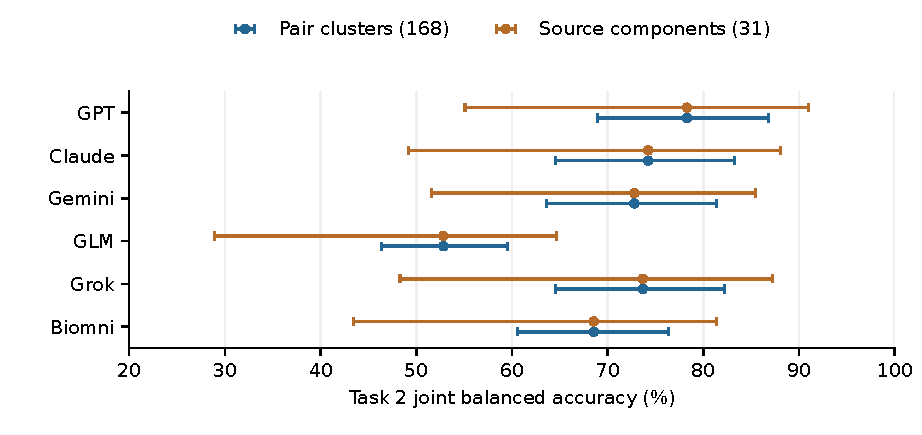
\includegraphics[width=.94\linewidth]{figs/cluster_intervals.pdf}
\caption{Task 2 joint balanced accuracy under two cluster assumptions. Dots show the unchanged published point estimate; bars are 95\% percentile intervals from 20,000 paired bootstrap draws. All units and four observed runs stay within the sampled cluster. Source components merge papers linked by shared pairs. Their wider intervals expose limited source diversity and do not incorporate judge uncertainty.}\label{fig:cluster_intervals}
\end{figure}
\begin{center}
\begin{tabular}{lrrrr}
\toprule
 & \multicolumn{2}{c}{Pair bootstrap} & \multicolumn{2}{c}{Source-component bootstrap} \\
System & Mean rank & First place (\%) & Mean rank & First place (\%) \\
\midrule
GPT & 1.02 & 97.97 & 1.13 & 88.54 \\
Claude & 2.58 & 1.98 & 2.84 & 6.79 \\
Gemini & 3.51 & 0.01 & 3.17 & 3.36 \\
GLM & 6.00 & 0.00 & 6.00 & 0.00 \\
Grok & 2.95 & 0.04 & 3.05 & 1.05 \\
Biomni & 4.94 & 0.00 & 4.81 & 0.25 \\
\bottomrule
\end{tabular}
\end{center}
Ties use midranks and split first-place credit. The entire original strict six-system ordering recurs in 36.35\% of pair draws and 18.96\% of source-component draws. GPT receives 97.97\% and 88.54\% of first-place credit. A comparatively frequent first place can coexist with uncertain adjacent ranks and a source-aware paired interval crossing zero. These frequencies describe this fixed benchmark, not the probability of a universal model ordering.

For the secondary equal-pair analysis, corrected tie-aware calculations retain the entire strict ordering in 52.76\% (chain) and 48.46\% (joint) of draws; mean Kendall $\tau_b$ is 0.924 and 0.921. Grok/Gemini invert in 28.70\% and 40.82\% of draws. Inversion counts compare the same systems in every draw, regardless of whether they remain adjacent. These calculations correct the supplied permutation-based rank comparison and adjacency-restricted flip counter without changing any pass-rate point estimate or interval.

\paragraph{Scope and reproducibility.} Per-pair dependence, source concentration, repeated-run variability and judge sensitivity are different uncertainty sources. This analysis addresses the first two while retaining observed runs; Appendix~\ref{app:judge_robustness} separately probes automated adjudication. Bootstrap intervals do not validate the biological labels or extrapolate to unseen TF families. The release includes source-component assignments, every bootstrap replicate, paired differences and all six-system rank summaries, together with deterministic reproduction scripts.

\clearpage
\endgroup
\end{document}

